%%%%%%%%%%%%%%%%%%%%%%%%%%%%%%%%%%%%%%%%%%%%%%%%%%%%%%%%%%%%%%%%%%%%%%%
% Latex file abstraction to pkl class
%%%%%%%%%%%%%%%%%%%%%%%%%%%%%%%%%%%%%%%%%%%%%%%%%%%%%%%%%%%%%%%%%%%%%%%
\documentclass{pkl}

% -----------------------------------------------------------------
% Font style
% -----------------------------------------------------------------
\usepackage{fontspec} % use custom font

\setmainfont{Calibri}[
    Path = /home/omar/.local/share/fonts/,
    Extension = .ttf,
    UprightFont = calibri-regular,
    BoldFont = calibri-bold,
    ItalicFont = calibri-italic
]

% ------------------------------------------------------------
% Add your own needed package here
% ------------------------------------------------------------
\usepackage[titles]{tocloft} % add prefix for images and tables
\renewcommand\cftfigpresnum{Gambar\  }
\renewcommand\cfttabpresnum{Tabel\   }

\usepackage[normalem]{ulem}
\usepackage{hyperref} % add hyperlink to the document
\urlstyle{same}
\usepackage{xurl}
\usepackage{tabularx}
\makeatletter
\def\UrlBreaks{%
  \do\/%
  \do\-%
  \do\_%
  \do\?%
  \do\&%
  \do\=%
  \do\.%
}
\makeatother
\newlength{\mylenf}
\settowidth{\mylenf}{\cftfigpresnum}
\setlength{\cftfignumwidth}{\dimexpr\mylenf+2em}
\setlength{\cfttabnumwidth}{\dimexpr\mylenf+2em}

\usepackage[labelfont=bf]{caption} % Bold Face for image description

\usepackage{caption} % add ability to customize caption
\captionsetup{
  labelsep=space
}

\usepackage{float}

\usepackage{placeins}

\usepackage{longtable}

\usepackage{subcaption} % add ability to customize subcaption
% - \usepackage{showframe} % show frame margin

\usepackage{graphicx}
% \setmainfont{Carlito} % carlito is calibri replacement

% -----------------------------------------------------------------
% Bibliography style
% -----------------------------------------------------------------
% \usepackage[style=authoryear, % author year style
% %\usepackage[style=agsm, % author year style
% firstinits=true, % abbrev fist name
% ]{biblatex}
% \DeclareNameAlias{author}{last-first} % put last name fist at
%                                 % bibliography list

\input{hangilastyle}
\addbibresource{daftar-pustaka.bib}

\renewcommand*{\finalnamedelim}{% % change and to &
  \ifnumgreater{\value{liststop}}{2}{\finalandcomma}{}%
  \addspace\&\space}

\newcommand{\cmmnt}[1]{\ignorespaces} % remove space in generated
% documents if we put comments in source

% -----------------------------------------------------------------
% Fill your data here
% -----------------------------------------------------------------
% title
\titlepkl{Implementasi Laravel Sebagai Framework Backend pada Aplikas Web SIPANTAU: Aplikasi Web Digital Model untuk Prediksi Harga Komoditas Fluktuatif}
% personal data
\fullname{Muhammad Omar Haqqi}
\idnum{235150219111001}
\approvaldate{11}
\degree{N/A}
\yearsubmit{2026}
\laboratory{Rekayasa Perangkat Lunak}
\pklplacetype{Pemerintah}
\pklstartdate{1 Juli}
\pklenddate{31 Agustus 2018}
\pklplace{Kabupaten Sukabumi}
\dept{TEKNIK INFORMATIKA}
\faculty{FAKULTAS ILMU KOMPUTER}
\university{universitas brawijaya}
\city{malang}
% supervisor data
\firstsupervisor{Nama Ketua Jurusan, S.T., M.T., Ph.D}
\firstsupervisornip{1234 45679}
\secondsupervisor{Nama Dosen Pembimbing, S.T., M.T., Ph.D}
\secondsupervisornip{5555 7777}
\thirdsupervisor{Abu al-Qasim al-Zahrawi}
\thirdsupervisornip{1111 2222}


% -----------------------------------------------------------------
% And so it begins
% -----------------------------------------------------------------
\begin{document}

% -----------------------------------------------------------------
% Cover
% -----------------------------------------------------------------
\cover

% -----------------------------------------------------------------
% Approval Page
% -----------------------------------------------------------------
% \approvalpage

% -----------------------------------------------------------------
% Approval Page Lapangan
% -----------------------------------------------------------------
% \approvalpagelapangan


%-----------------------------------------------------------------
%Disini awal masukan untuk Prakata
%-----------------------------------------------------------------
% \preface

% Puji syukur kehadirat Allah SWT yang telah melimpahkan
% rahmat, taufik dan hidayah-Nya sehingga laporan PKL yang berjudul
% “Pembuatan Aplikasi Web Digital Twin untuk Prediksi Harga Komoditas
% Fluktuatif dengan Laravel Sebagai Framework Backend” ini dapat terselesaikan.

% \begin{enumerate}
% \item{Bapak Nama Pembimbing, S.Si., M.Sc. selaku dosen pembimbing PKL
%     yang telah dengan sabar membimbing dan mengarahkan penulis
%     sehingga dapat menyelesaikan laporan ini.}
% \item{Bapak Drs. Ketua Program Studi, M.Kom. selaku ketua Program
%     Studi Teknik Informatika.}
% \item{Bapak Nama Ketua Jurusan, S.T., M.T., Ph.D. selaku selaku ketua
%     Jurusan Teknik Informatika.}
% \item{Ayahanda dan Ibunda dan seluruh keluarga besar atas segala
%     nasehat, kasih sayang, perhatian dan kesabarannya di dalam
%     membesarkan dan mendidik penulis, serta yang senantiasa tiada
%     henti-hentinya memberikan doa dan semangat demi terselesaikannya
%     laporan ini.}
% \item{Seluruh civitas akademika Teknik Informatika Universitas
%     Brawijaya yang telah banyak memberi bantuan dan dukungan selama
%     penyelesaian laporan PKL ini.}
% \end{enumerate}

% Penulis menyadari bahwa dalam penyusunan laporan ini masih banyak kekurangan,
% sehingga saran dan kritik yang membangun sangat penulis harapkan. Akhir kata penulis
% berharap PKL ini dapat membawa manfaat bagi semua pihak yang menggunakannya.

% \vspace{1.5cm}

% \begin{tabular}{p{7.5cm}c}
% &Malang, 1 Juli 2017\\
% &\\
% &\\
% &{Penulis}
% \end{tabular}

% -----------------------------------------------------------------
% TOCS
% -----------------------------------------------------------------
\tableofcontents
\addcontentsline{toc}{chapter}{DAFTAR ISI}
\listoftables
\addcontentsline{toc}{chapter}{DAFTAR TABEL}
\listoffigures
\addcontentsline{toc}{chapter}{DAFTAR GAMBAR}
% \listofappendices TODO
\addcontentsline{toc}{chapter}{DAFTAR LAMPIRAN}

% -----------------------------------------------------------------
% Chapter
% -----------------------------------------------------------------
% change numbering to arabic from bab1
\selectlanguage{bahasa}\clearpage\pagenumbering{arabic}\setcounter{page}{1}

%%%%%%%%%%%%%%%%%%%%%%%%%%%%%%%%%%%%%%%%%%%%%%%%%%%%%%%%%%%%%%%%%%%%%%%
% BAB 1
%%%%%%%%%%%%%%%%%%%%%%%%%%%%%%%%%%%%%%%%%%%%%%%%%%%%%%%%%%%%%%%%%%%%%%%
\mychapter{1}{BAB 1 PENDAHULUAN}

\section{Latar Belakang}

Kabupaten Sukabumi merupakan salah satu wilayah dengan luas daratan terbesar di Jawa Barat \parencite{bps-luas-2025} dengan sektor Pertanian, Kehutanan, dan Perikanan sebagai kontributor terbesar terhadap perekonomian daerah dengan kontribusi sebesar 24,27\% dan secara konsisten menjadi sektor dengan kontribusi tertinggi selama periode 2021–2025 \parencite{bps-sukabumi-2026}. Aktivitas distribusi komoditas pangan antarkecamatan menjadi salah satu faktor penting dalam menjaga ketersediaan pasokan dan stabilitas harga bahan pokok. Dengan jumlah penduduk mencapai lebih dari 2,6 juta jiwa dan 47 kecamatan yang tersebar mulai dari wilayah pegunungan hingga pesisir selatan \parencite{bps-penduduk-2025}, stabilitas harga bahan pokok menjadi tantangan utama dalam menjaga kesejahteraan masyarakat.

Komoditas pangan strategis termasuk ke dalam kelompok volatile food, yaitu komoditas yang memiliki karakteristik harga cenderung berfluktuasi. Kelompok komoditas tersebut meliputi beras, daging ayam, daging sapi, telur ayam, bawang merah, bawang putih, cabai merah, cabai rawit, minyak goreng, dan gula pasir \parencite{Helbawanti_Saputro_Ulfa_2021}. Kondisi tersebut juga terlihat pada data harga harian cabai rawit merah Kabupaten Sukabumi selama periode Januari 2025 hingga April 2026, di mana harga komoditas tersebut berubah dari sekitar Rp28.000/kg hingga mencapai Rp100.000/kg \parencite{data-pemerintah}. Fluktuasi harga tersebut menunjukkan bahwa komoditas pangan memiliki karakteristik yang dinamis sehingga diperlukan sistem yang mampu memantau sekaligus memprediksi pergerakan harga berdasarkan data historis.

Fluktuasi harga komoditas pangan yang tinggi menunjukkan bahwa informasi harga aktual saja belum cukup untuk mendukung proses pengambilan keputusan. Prediksi harga komoditas pertanian menjadi masukan penting bagi berbagai pemangku kepentingan, termasuk pemerintah, dalam merencanakan kebijakan, menjaga stabilitas pasokan, serta mendukung kesejahteraan masyarakat. Oleh karena itu, diperlukan suatu sistem yang mampu melakukan prediksi harga secara akurat berdasarkan data historis dan faktor-faktor yang memengaruhinya sehingga dapat menghasilkan informasi yang lebih bernilai dibandingkan sekadar penyajian data harga saat ini \parencite{bhardwaj2023innovativedeeplearningbased}.

Berdasarkan permasalahan tersebut, diperlukan suatu sistem yang dapat mendukung proses pemantauan harga komoditas pangan secara berkelanjutan melalui pemanfaatan data historis. Sistem tersebut diharapkan mampu mengintegrasikan proses pengumpulan data harga pasar, harga petani, serta data ketersediaan dan kebutuhan harian dari instansi terkait sebagai masukan bagi layanan prediksi harga. Hasil prediksi tersebut kemudian disajikan kepada Tim Pengendalian Inflasi Daerah (TPID) sebagai informasi pendukung dalam kegiatan pemantauan harga dan pengambilan keputusan. Oleh karena itu, dikembangkan Sistem Informasi Pemantauan Harga Komoditas (SIPANTAU) berbasis web sebagai media yang mengintegrasikan proses pengumpulan data dan penyajian hasil prediksi harga komoditas pangan di Kabupaten Sukabumi.

% Lorem ipsum dolor sit amet, consectetur adipiscing elit. Quisque
% tincidunt tellus sit amet tincidunt lobortis. Nulla id tempus
% enim. Curabitur sed enim quam. Duis suscipit in nibh nec
% gravida. Curabitur placerat ullamcorper dolor a rhoncus. Duis ac
% suscipit enim. Ut elementum tortor ligula, fringilla viverra diam
% varius eget. Vivamus quis iaculis lorem. Vivamus nec dignissim libero,
% eu congue sem. Nam id lobortis elit \parencite{foster}.

% Phasellus porttitor purus \textcite{warn} vitae finibus laoreet. Class
% aptent taciti sociosqu ad litora torquent per conubia nostra, per
% inceptos himenaeos. Lorem ipsum dolor sit amet, consectetur adipiscing
% elit. Nunc tempus sed purus sit amet porta. Sed volutpat est ac arcu
% porttitor, non pharetra tortor pharetra. Phasellus vitae dictum
% elit. Curabitur elementum consequat elementum. Integer in vulputate
% metus. Aliquam erat volutpat. Phasellus vitae convallis orci. Etiam ac
% metus tristique, viverra metus a, mattis lectus. Aenean vel vestibulum
% augue.

\section{Rumusan Masalah}

% Phasellus porttitor purus vitae finibus laoreet. Class aptent taciti
% sociosqu ad litora torquent per conubia nostra, per inceptos
% himenaeos. Lorem ipsum dolor sit amet, consectetur adipiscing
% elit. Nunc tempus sed purus sit amet porta. Sed volutpat est ac arcu
% porttitor, non pharetra tortor pharetra. Phasellus vitae dictum
% elit. Curabitur elementum consequat elementum. Integer in vulputate
% metus. Aliquam erat volutpat. Phasellus vitae convallis orci. Etiam ac
% metus tristique, viverra metus a, mattis lectus. Aenean vel vestibulum
% augue.

\begin{enumerate}
\item Bagaimana membangun website SIPANTAU yang mendukung proses pengumpulan data harga komoditas pangan dari instansi terkait sebagai dasar prediksi harga?
\item Bagaimana menyediakan hasil prediksi harga komoditas pangan untuk tiga hari ke depan melalui website SIPANTAU sebagai pendukung kegiatan pemantauan harga oleh TPID?
\end{enumerate}


\section{Tujuan}

\begin{enumerate}
\item Membangun website SIPANTAU yang mendukung proses pengumpulan data harga komoditas pangan dari instansi terkait sebagai dasar prediksi harga.
\item Menyediakan hasil prediksi harga komoditas pangan untuk tiga hari ke depan melalui website SIPANTAU sebagai pendukung kegiatan pemantauan harga oleh TPID.
\end{enumerate}


\section{Manfaat}

\begin{enumerate}
\item Pemerintah Kabupaten Sukabumi (Dinas terkait) \par
Membantu Dinas Pertanian, Dinas Perdagangan, dan Dinas Ketahanan Pangan dalam melakukan pengelolaan serta pembaruan data harga komoditas dan data pendukung secara terpusat sehingga dapat digunakan sebagai dasar proses prediksi harga komoditas pangan.
\item Tim Pengendali Inflasi Daerah \par
Memberikan informasi hasil prediksi harga komoditas pangan sebagai bahan pendukung dalam proses pemantauan harga serta pengambilan keputusan terkait pengendalian inflasi dan stabilisasi harga.
\item Penulis \par
Menambah pengalaman dalam pengembangan layanan backend berbasis web menggunakan framework Laravel, pengelolaan basis data MySQL, integrasi layanan prediksi, serta proses deployment aplikasi pada lingkungan server.
\end{enumerate}

% Curabitur elementum consequat elementum. Integer in vulputate
% metus. Aliquam erat volutpat. Phasellus vitae convallis orci. Etiam ac
% metus tristique, viverra metus a, mattis lectus. Aenean vel vestibulum
% augue.


\section{Batasan Masalah}

\begin{enumerate}
\item Sistem yang dibahas adalah Sistem Informasi Pemantauan Harga Komoditas (SIPANTAU) pada lingkup Kabupaten Sukabumi.
\item Data yang digunakan merupakan data harga pasar, harga petani, data ketersediaan dan kebutuhan harian, dan data panen komoditas pangan yang diperoleh dari Pemerintah Kabupaten Sukabumi sebagai data internal.
\item Komoditas yang dianalisis dalam sistem ini dibatasi pada beberapa komoditas strategis, yaitu cabai rawit merah, cabai merah besar, bawang merah, dan beras.
\item Implementasi sistem difokuskan pada wilayah Pasar Cisaat sebagai studi kasus selama periode pelaksanaan Praktik Kerja Lapang untuk memastikan sistem berjalan secara fungsional.
\item Sistem berfokus pada proses pengumpulan data, integrasi layanan prediksi harga, dan penyajian hasil prediksi, serta tidak mencakup pengembangan model prediksi maupun implementasi kebijakan pemerintah secara langsung.
\item Sistem menggunakan pembagian hak akses (\emph{role-based access control}), yaitu Dinas (Pertanian, Perdagangan, dan Ketahanan Pangan) sebagai pengelola dan input data, serta TPID sebagai pengguna fitur analisis dan prediksi.
\item Integrasi data eksternal melalui API (seperti SILINDA) masih dalam tahap pengembangan dan belum diimplementasikan pada sistem saat ini.
\item Model prediksi harga merupakan layanan yang telah tersedia dan tidak menjadi bagian dari pengembangan pada kegiatan Praktik Kerja Lapang ini. Ruang lingkup pengembangan difokuskan pada integrasi layanan prediksi ke dalam website SIPANTAU melalui backend.
\end{enumerate}


% \section{Sistematika Pembahasan}
% \noindent
% \textbf{BAB I : PENDAHULUAN}

% Pada bab ini dijelaskan latar belakang, rumusan masalah, batasan,
% tujuan, manfaat,  dan sistematika penulisan.\\

% \noindent
% \textbf{BAB II : TINJAUAN PUSTAKA DAN LANDASAN TEORI}

% Pada bab ini dijelaskan teori-teori dan penelitian terdahulu yang
% digunakan sebagai acuan dan dasar dalam penelitian.\\

% \noindent
% \textbf{BAB III : METODOLOGI PENELITIAN}

% Pada bab ini dijelaskan metode yang digunakan dalam penelitian
% meliputi langkah kerja, pertanyaan penilitian, alat dan bahan, serta
% tahapan dan alur penelitian.\\

% \noindent
% \textbf{BAB IV : HASIL DAN PEMBAHASAN}

% Pada bab ini dijelaskan hasil penelitian dan pembahasannya.\\

% \noindent
% \textbf{BAB V : KESIMPULAN DAN SARAN}

% Pada bab ini ditulis kesimpulan akhir dari penelitian dan saran untuk
% pengembangan penelitian selanjutnya.\\

%%%%%%%%%%%%%%%%%%%%%%%%%%%%%%%%%%%%%%%%%%%%%%%%%%%%%%%%%%%%%%%%%%%%%%%
% BAB 2
%%%%%%%%%%%%%%%%%%%%%%%%%%%%%%%%%%%%%%%%%%%%%%%%%%%%%%%%%%%%%%%%%%%%%%%

\mychapter{2}{BAB 2 PROFIL OBYEK PKL}

% Curabitur elementum consequat elementum. Integer in vulputate
% metus. Aliquam erat volutpat. Phasellus vitae convallis orci. Etiam ac
% metus tristique, viverra metus a, mattis lectus. Aenean vel vestibulum
% augue.

\section{Sejarah}

Sejarah Kabupaten Sukabumi berkaitan dengan perkembangan wilayah administratif Sukabumi pada masa pemerintahan Hindia Belanda. Berdasarkan hasil penelusuran sejarah yang menjadi dasar penetapan hari jadi Kabupaten Sukabumi, keberadaan Sukabumi telah tercatat dalam keputusan Gubernur Jenderal P. Meijer pada tanggal 10 September 1870. Keputusan tersebut membagi wilayah Afdeeling Cianjur menjadi dua wilayah administratif, yaitu Afdeeling Cianjur dan Afdeeling Sukabumi. Berdasarkan keputusan tersebut, tanggal 10 September 1870 kemudian ditetapkan sebagai Hari Jadi Kabupaten Sukabumi melalui Peraturan Daerah Kabupaten Sukabumi Nomor 14 Tahun 2018 \parencite{perda14_2018}.

Perkembangan Kabupaten Sukabumi kemudian berlanjut hingga menjadi kabupaten mandiri. Berdasarkan \textit{Profil Perkembangan Kependudukan Kabupaten Sukabumi Tahun 2025}, Kabupaten Sukabumi resmi berdiri sebagai kabupaten mandiri pada tanggal 1 Juni 1921 setelah terlepas dari Kabupaten Cianjur, dengan pusat pemerintahan awal berada di Tjikole. Dokumen tersebut juga menyebutkan bahwa nama Soekaboemi telah digunakan sejak 13 Januari 1815 dan dikaitkan dengan wilayah perkebunan kopi pada masa tersebut \parencite{disdukcapil2026}.

Dalam perkembangannya, Kabupaten Sukabumi menjadi salah satu wilayah administratif di Provinsi Jawa Barat. Pusat pemerintahan Kabupaten Sukabumi saat ini berada di Palabuhanratu. Perkembangan wilayah dan penyelenggaraan pemerintahan Kabupaten Sukabumi menjadi bagian dari perjalanan administratif daerah hingga terbentuknya Pemerintah Kabupaten Sukabumi sebagaimana dikenal saat ini \parencite{disdukcapil2026}.

% \section{Profil}

% % comments
% %% comments
% Sekretariat Daerah Kabupaten Sukabumi merupakan unsur staf pemerintah daerah yang mempunyai tugas membantu Bupati dalam penyusunan kebijakan, pengoordinasian administratif terhadap pelaksanaan tugas perangkat daerah, serta penyelenggaraan pelayanan administratif. Dalam menjalankan tugas tersebut, Sekretariat Daerah berfungsi sebagai unsur pendukung dalam perumusan kebijakan daerah, koordinasi pelaksanaan pembangunan, serta penyelenggaraan pelayanan administrasi pemerintahan \parencite{renstra_setda_2021}.

% Bagian Perekonomian merupakan salah satu bagian yang berada di bawah Asisten Perekonomian dan Pembangunan pada Sekretariat Daerah Kabupaten Sukabumi. Bagian ini mempunyai tugas melaksanakan sebagian fungsi Asisten Perekonomian dan Pembangunan dalam pengoordinasian perumusan kebijakan daerah, pengoordinasian pelaksanaan tugas perangkat daerah, serta pemantauan dan evaluasi kebijakan di bidang pembinaan BUMD dan BLUD, pengendalian dan distribusi perekonomian, serta perencanaan dan pengawasan ekonomi mikro kecil. Selain itu, Bagian Perekonomian juga mengoordinasikan beberapa perangkat daerah, di antaranya Dinas Pertanian, Dinas Peternakan, Dinas Ketahanan Pangan, Dinas Perikanan, Dinas Koperasi, Usaha Kecil dan Menengah, Dinas Perdagangan dan Perindustrian, serta Dinas Penanaman Modal dan Pelayanan Terpadu Satu Pintu \parencite{perbup1002021,web_setda}.

% Dalam kegiatan Praktik Kerja Lapang, penulis ditempatkan pada Bagian Perekonomian Sekretariat Daerah Kabupaten Sukabumi dan terlibat dalam pengembangan layanan backend pada Sistem Informasi Pemantauan Harga Komoditas (SIPANTAU). Sistem tersebut dikembangkan untuk mendukung koordinasi antardinas dalam proses pengumpulan data harga komoditas serta penyajian hasil prediksi harga sebagai informasi pendukung bagi Tim Pengendalian Inflasi Daerah (TPID).

\section{Alamat}

Jl. Siliwangi No. 10, Kecamatan Palabuhanratu, Kabupaten Sukabumi, Jawa Barat 43164

% \subsection{\emph{Lorem}}
% \label{subsec:label}

% Bagian Perekonomian merupakan salah satu bagian yang berada di lingkungan Sekretariat Daerah Kabupaten Sukabumi. Kantor Bagian Perekonomian berlokasi di Jalan Siliwangi No. 10, Kecamatan Palabuhanratu, Kabupaten Sukabumi, Jawa Barat 43164. Lokasi tersebut berada di kawasan Komplek Perkantoran Pemerintah Kabupaten Sukabumi dan menjadi pusat pelaksanaan berbagai kegiatan administrasi serta koordinasi pemerintahan, termasuk koordinasi di bidang perekonomian daerah \parencite{web_setda}.

% \begin{table}[ht]
%     \centering
%     \caption{\textbf{Informasi Umum Bagian Perekonomian Sekretariat Daerah Kabupaten Sukabumi}}
%     \label{tab:informasi-instansi}

%     \begin{tabular}{|p{4cm}|p{10cm}|}
%         \hline
%         Keterangan & Informasi \\
%         \hline
%         Nama Instansi &
%         Bagian Perekonomian Sekretariat Daerah Kabupaten Sukabumi \\
%         \hline

%         Alamat &
%         Jl. Siliwangi No. 10, Kecamatan Palabuhanratu, Kabupaten Sukabumi, Jawa Barat 43164 \\
%         \hline

%         Kode Plus &
%         2H72+38 Palabuhanratu, Kabupaten Sukabumi, Jawa Barat \\
%         \hline

%         Website &
%         \url{https://setda.sukabumikab.go.id} \\
%         \hline
%     \end{tabular}
% \end{table}

\section{Visi dan Misi}

\subsection{Visi}
Mewujudkan Sukabumi yang Mubarakah (Maju, Unggul, Berbudaya, dan Berkah).

\subsection{Misi}
\begin{enumerate}
    \item Meningkatkan pertumbuhan ekonomi yang berkualitas dan berkelanjutan melalui pengembangan agroindustri dan pariwisata.

    \item Membangun infrastruktur pelayanan dasar dan penunjang perekonomian yang merata dan inklusif.

    \item Membangun sumber daya manusia yang unggul, berbudaya, berbasis Iptek dan Imtaq.

    \item Membangun pemerintahan yang kolaboratif, profesional dan akuntabel.
\end{enumerate}

% \section{Tugas dan Fungsi}

% Bagian Perekonomian merupakan salah satu bagian yang berada di bawah Asisten Perekonomian dan Pembangunan pada Sekretariat Daerah Kabupaten Sukabumi. Berdasarkan Peraturan Bupati Kabupaten Sukabumi Nomor 100 Tahun 2021 tentang Struktur Organisasi dan Tata Kerja Sekretariat Daerah, Bagian Perekonomian mempunyai tugas melaksanakan sebagian fungsi Asisten Perekonomian dan Pembangunan dalam pelaksanaan pengoordinasian perumusan kebijakan daerah, pengoordinasian pelaksanaan tugas perangkat daerah, serta pemantauan dan evaluasi pelaksanaan kebijakan daerah di bidang pembinaan Badan Usaha Milik Daerah (BUMD), Badan Layanan Umum Daerah (BLUD), pengendalian dan distribusi perekonomian, serta perencanaan dan pengawasan ekonomi mikro kecil \parencite{perbup1002021}.

% Dalam melaksanakan tugas tersebut, Bagian Perekonomian juga mengoordinasikan berbagai perangkat daerah yang berkaitan dengan bidang perekonomian, di antaranya Dinas Pertanian, Dinas Peternakan, Dinas Ketahanan Pangan, Dinas Perikanan, Dinas Koperasi, Usaha Kecil dan Menengah, Dinas Perdagangan dan Perindustrian, serta Dinas Penanaman Modal dan Pelayanan Terpadu Satu Pintu. Selain itu, Bagian Perekonomian melaksanakan kegiatan pemantauan dan evaluasi pelaksanaan kebijakan daerah sebagai bahan penyusunan rekomendasi kebijakan di bidang perekonomian \parencite{perbup1002021}.

% \begin{enumerate}
%     \item Menyusun rencana dan program kerja di bidang perekonomian.
%     \item Mengoordinasikan perumusan kebijakan daerah di bidang pembinaan BUMD, BLUD, pengendalian dan distribusi perekonomian, serta ekonomi mikro kecil.
%     \item Mengoordinasikan pelaksanaan tugas perangkat daerah di bidang perekonomian.
%     \item Melaksanakan pemantauan dan evaluasi terhadap pelaksanaan kebijakan daerah di bidang perekonomian.
%     \item Menyusun laporan pelaksanaan tugas dan melaksanakan fungsi lain yang diberikan oleh Asisten Perekonomian dan Pembangunan.
% \end{enumerate}

\section{Struktur Organisasi}

Struktur organisasi Pemerintah Kabupaten Sukabumi terdiri atas berbagai perangkat daerah yang mendukung penyelenggaraan urusan pemerintahan daerah. Berdasarkan Peraturan Daerah Kabupaten Sukabumi Nomor 7 Tahun 2021, perangkat daerah Pemerintah Kabupaten Sukabumi meliputi Sekretariat Daerah, Sekretariat DPRD, Inspektorat, Dinas, dan Badan. Sekretariat Daerah mempunyai tugas membantu Bupati dalam penyusunan kebijakan, pengoordinasian administratif terhadap pelaksanaan tugas perangkat daerah, serta pelayanan administratif. Sementara itu, Dinas merupakan unsur pelaksana urusan pemerintahan yang menjadi kewenangan daerah, sedangkan Badan merupakan unsur penunjang urusan pemerintahan daerah \parencite{perda7_2021}.

Dalam pelaksanaan Praktik Kerja Lapang, penulis ditempatkan di lingkungan Pemerintah Kabupaten Sukabumi pada Sekretariat Daerah, khususnya Bagian Perekonomian. Bagian Perekonomian merupakan bagian yang berada dalam koordinasi Asisten Perekonomian dan Pembangunan. Struktur organisasi Sekretariat Daerah Kabupaten Sukabumi yang menunjukkan posisi Bagian Perekonomian dapat dilihat pada Gambar \ref{fig:struktur-setda}.

\begin{figure}[H]
    \centering
    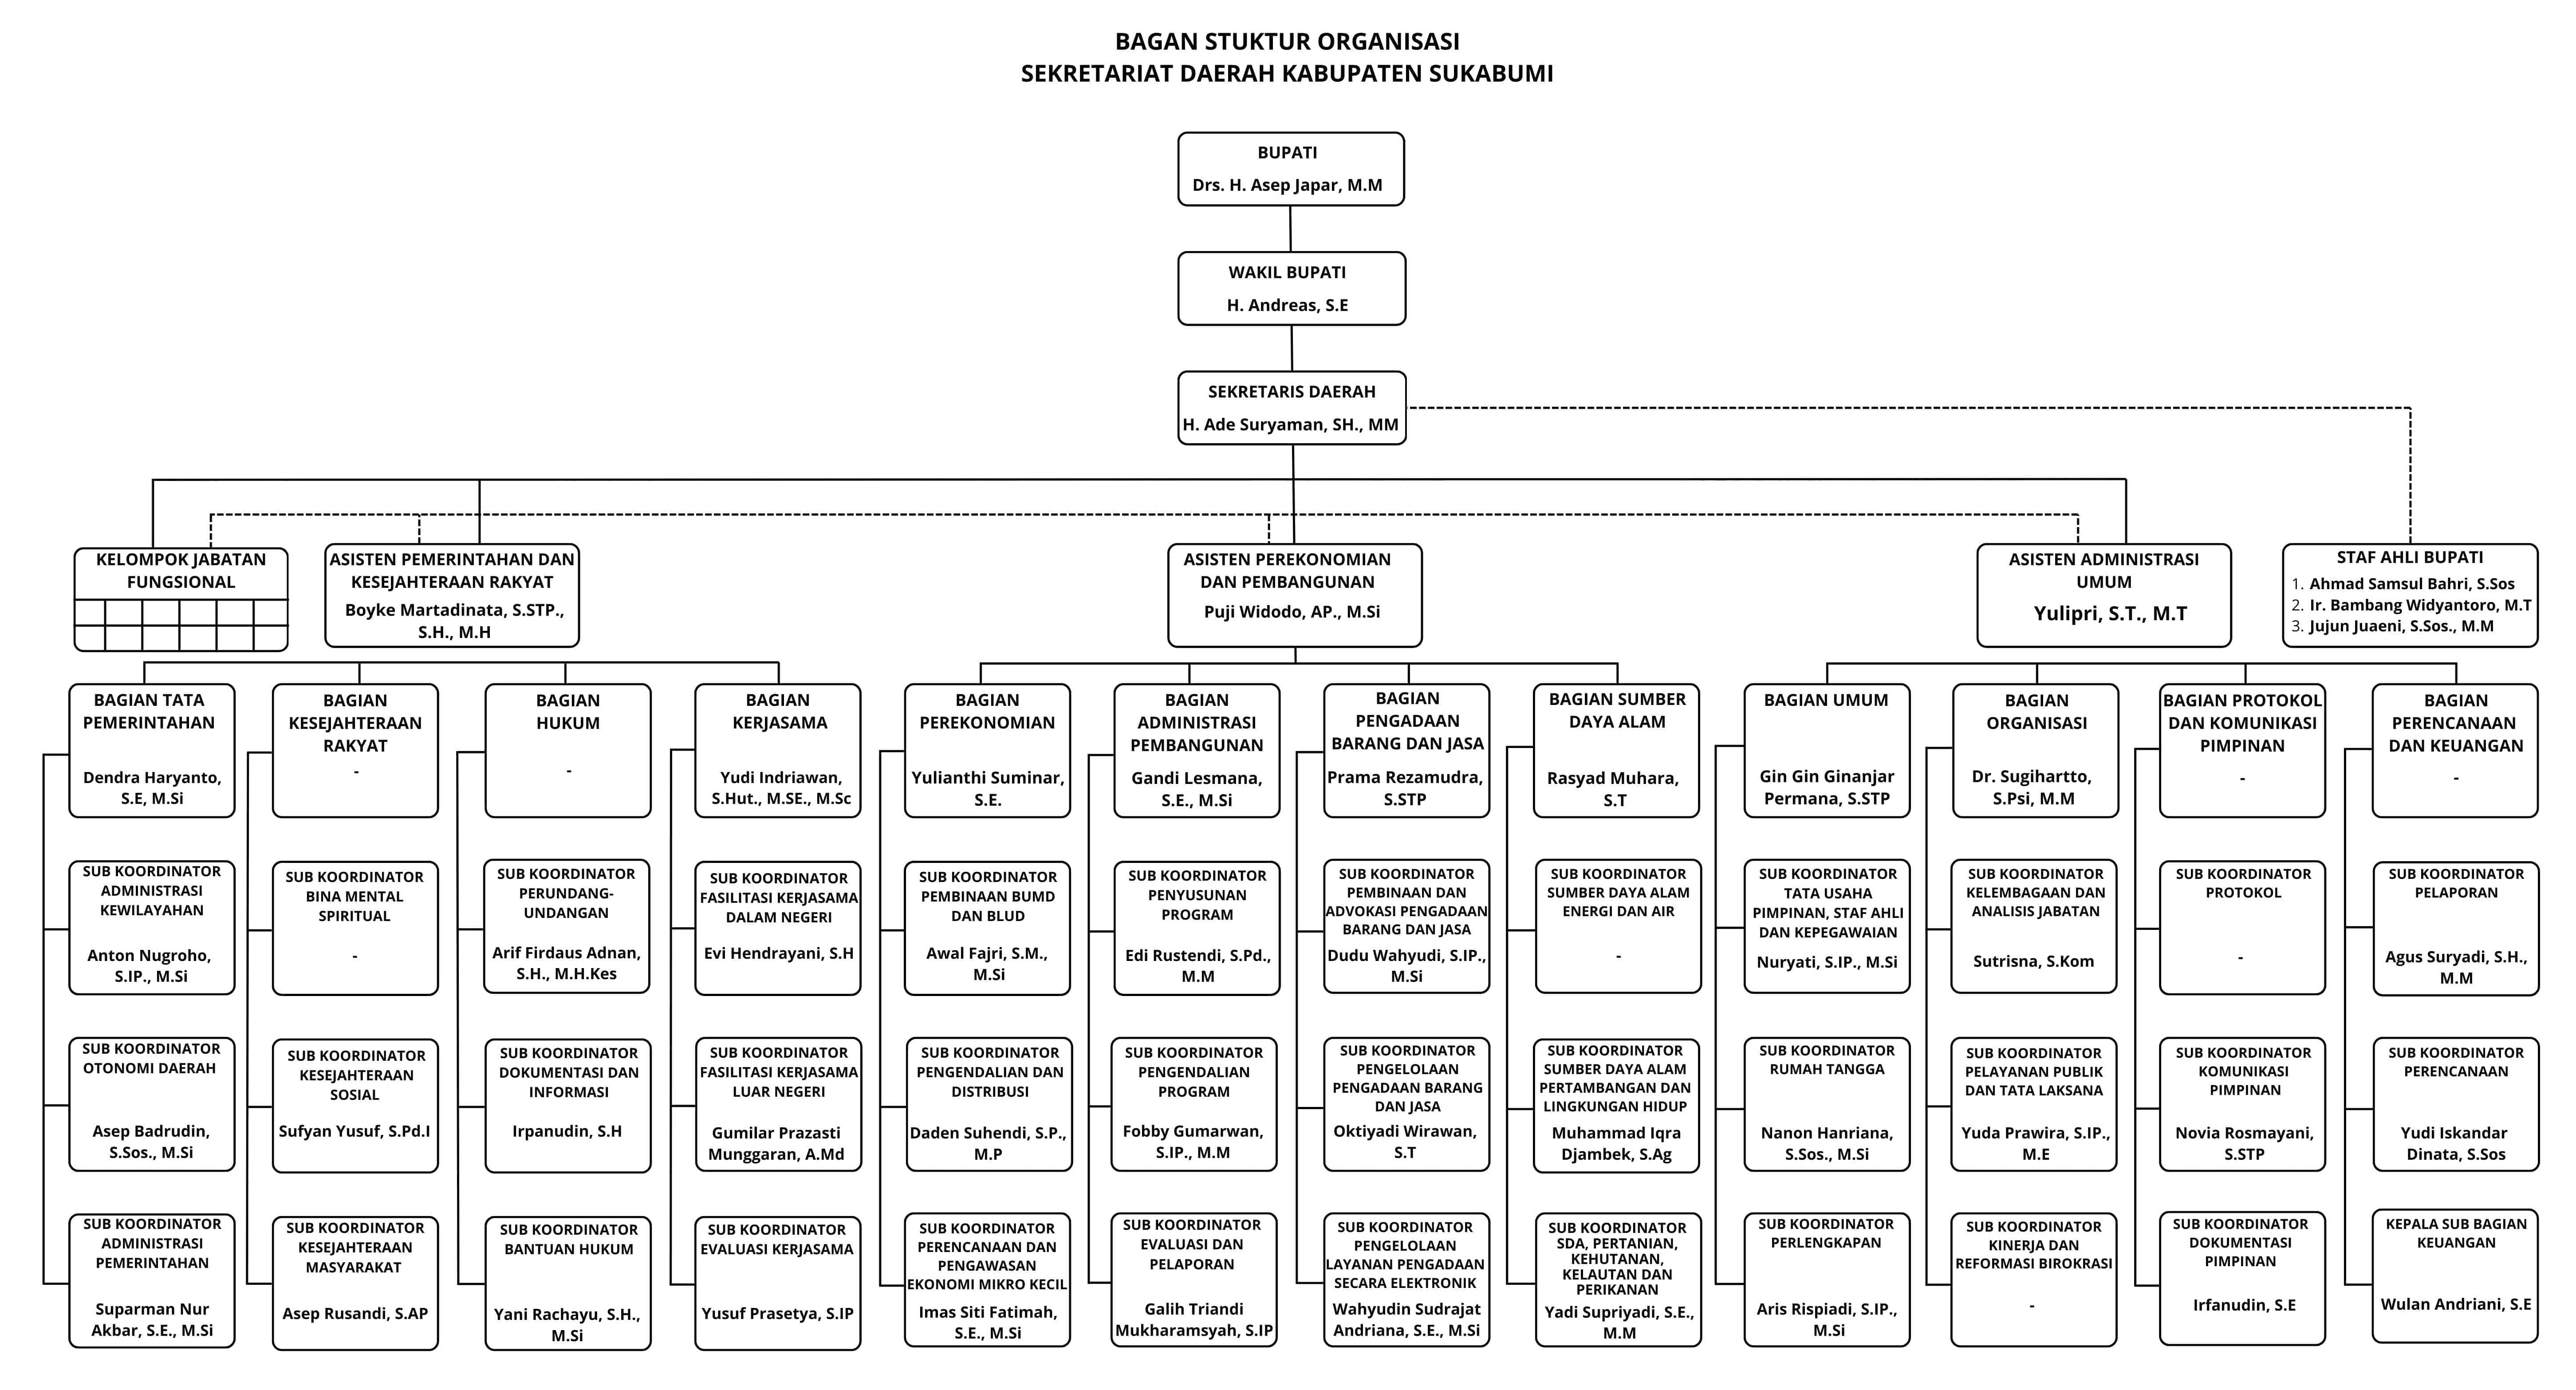
\includegraphics[width=\textwidth]{img/struktur_setda.jpg}
    \caption{Struktur Organisasi Sekretariat Daerah Kabupaten Sukabumi}
    \label{fig:struktur-setda}
\end{figure}

\section{Rantai Bisnis}

Rantai bisnis Pemerintah Kabupaten Sukabumi mencakup serangkaian aktivitas pemerintahan yang saling terintegrasi dalam mendukung penyelenggaraan urusan pemerintahan dan pelayanan kepada masyarakat. Proses tersebut diawali dengan perumusan kebijakan daerah yang menjadi dasar dalam menentukan arah pelaksanaan program dan kegiatan pemerintah daerah. Dalam proses ini, Sekretariat Daerah memiliki peran dalam membantu Bupati dalam penyusunan kebijakan serta melakukan pengoordinasian administratif terhadap pelaksanaan tugas perangkat daerah.

Tahap berikutnya adalah koordinasi pelaksanaan kebijakan dan tugas perangkat daerah sesuai dengan bidang masing-masing. Koordinasi tersebut dilakukan untuk memastikan pelaksanaan urusan pemerintahan dapat berjalan secara terarah dan sesuai dengan kebijakan yang telah ditetapkan. Pada bidang perekonomian, koordinasi dilaksanakan melalui Asisten Perekonomian dan Pembangunan serta Bagian Perekonomian yang memiliki tugas dalam pengoordinasian perumusan kebijakan, pengoordinasian pelaksanaan tugas perangkat daerah, serta pemantauan dan evaluasi kebijakan daerah di bidang perekonomian \parencite{perbup1002021}.

Pelaksanaan kebijakan selanjutnya dilakukan oleh perangkat daerah sesuai dengan tugas dan kewenangannya. Dalam bidang perekonomian, Bagian Perekonomian melakukan koordinasi dengan berbagai perangkat daerah, antara lain Dinas Ketahanan Pangan, Dinas Koperasi, Usaha Kecil dan Menengah, Dinas Perdagangan dan Perindustrian (Bidang Non Energi Sumber Daya Mineral), Dinas Penanaman Modal dan Pelayanan Terpadu Satu Pintu, Dinas Pariwisata, Dinas Perhubungan, dan Dinas Komunikasi, Informatika dan Persandian. Masing-masing perangkat daerah melaksanakan urusan pemerintahan sesuai dengan bidangnya, sedangkan Bagian Perekonomian menjalankan fungsi koordinasi dan fasilitasi terhadap pelaksanaan urusan tersebut \parencite{perbup1002021}.

Setelah pelaksanaan kebijakan dan program berjalan, dilakukan proses pemantauan dan evaluasi untuk mengetahui pencapaian tujuan kebijakan, dampak yang ditimbulkan, serta faktor-faktor yang memengaruhi pencapaian kebijakan. Kegiatan tersebut menjadi bagian dari fungsi Bagian Perekonomian dalam melakukan pemantauan dan evaluasi pelaksanaan kebijakan daerah di bidang perekonomian. Hasil pemantauan dan evaluasi selanjutnya menjadi bagian dari proses pelaporan serta dapat digunakan sebagai bahan dalam melakukan tindak lanjut dan penyempurnaan pelaksanaan kebijakan daerah \parencite{perbup1002021}. Dengan demikian, rantai bisnis Pemerintah Kabupaten Sukabumi berlangsung secara berkelanjutan melalui tahapan perumusan kebijakan, koordinasi, pelaksanaan urusan pemerintahan, pemantauan dan evaluasi, serta pelaporan dan tindak lanjut.

% \subsection{\emph{Ipsum}}
% \label{subsec:label}

% Curabitur elementum consequat elementum. Integer in vulputate
% metus. Aliquam erat volutpat. Phasellus vitae convallis orci. Etiam ac
% metus tristique, viverra metus a, mattis lectus. Aenean vel vestibulum
% augue.

% \subsection{\emph{Dolor sit}}
% \label{subsec:label}

% Curabitur elementum consequat elementum. Integer in vulputate
% metus. Aliquam erat volutpat. Phasellus vitae convallis orci. Etiam ac
% metus tristique, viverra metus a, mattis lectus. Aenean vel vestibulum
% augue.


% % TODO
% % dolor
% % sit

% \section{Teknologi Pengembangan Perangkat Lunak}

% \subsection{\emph{Curabitur}}

% Curabitur elementum consequat elementum. Integer in vulputate
% metus. Aliquam erat volutpat. Phasellus vitae convallis orci. Etiam ac
% metus tristique, viverra metus a, mattis lectus. Aenean vel vestibulum
% augue.

% \subsection{\emph{Elementum}}

% Curabitur elementum consequat elementum. Integer in vulputate
% metus. Aliquam erat volutpat. Phasellus vitae convallis orci. Etiam ac
% metus tristique, viverra metus a, mattis lectus. Aenean vel vestibulum
% augue.

%%%%%%%%%%%%%%%%%%%%%%%%%%%%%%%%%%%%%%%%%%%%%%%%%%%%%%%%%%%%%%%%%%%%%%%
% BAB 3
%%%%%%%%%%%%%%%%%%%%%%%%%%%%%%%%%%%%%%%%%%%%%%%%%%%%%%%%%%%%%%%%%%%%%%%

\mychapter{3}{BAB 3 TINJAUAN PUSTAKA}

% Donec vitae rutrum arcu. Aenean dictum mauris id lobortis
% vulputate. In ut pretium turpis. Nunc elit nunc, blandit et maximus
% at, maximus at orci. Aliquam a nisl pretium, eleifend odio sit amet,
% interdum augue. Donec magna elit, cursus gravida libero vitae, congue
% luctus sapien. Phasellus sit amet nisl sed nisl dictum
% porttitor. Etiam viverra lacus est, a ultrices nisi euismod ut.

\section{Aplikasi Web}
% \label{subsec:label}

Website merupakan kumpulan halaman Web yang saling berkaitan dan umumnya berada pada server yang sama serta memuat informasi yang disediakan oleh individu, kelompok, maupun organisasi. Website digunakan sebagai salah satu media untuk menyampaikan berbagai informasi kepada pengguna melalui jaringan Internet \parencite{Laksono2021}. Sejalan dengan pengertian tersebut, Kulakat, Utami, dan Wibowo menjelaskan bahwa website merupakan kumpulan dokumen daring yang berisi halaman Web dan terikat pada suatu domain sehingga dapat diakses oleh pengunjung melalui Internet. Informasi yang terdapat pada website dapat diakses oleh pengguna melalui halaman Web yang tersedia \parencite{Kulakat2021}.

Pada perkembangannya, website tidak hanya digunakan sebagai media penyampaian informasi yang bersifat statis, tetapi telah berkembang menjadi media yang lebih dinamis dan interaktif. Website dapat menyediakan berbagai fungsi sesuai dengan kebutuhan pengguna, seperti pengelolaan dan penyampaian data. Perkembangan tersebut didukung oleh penggunaan berbagai bahasa pemrograman dan teknologi pengembangan website, seperti HTML, PHP, CSS, JavaScript, serta basis data MySQL \parencite{Purbo2021}.

Pengembangan website dapat memanfaatkan framework untuk membantu proses pembangunan aplikasi. Framework menyediakan struktur dan fungsi yang dapat digunakan kembali sehingga pengembang tidak perlu membangun seluruh komponen aplikasi dari awal. Penggunaan framework juga dapat membantu pengembangan website menjadi lebih terstruktur dan mempermudah proses pengembangan serta pemeliharaan aplikasi \parencite{Purbo2021}.

% Dalam konteks pengembangan SIPANTAU, website digunakan sebagai media penyediaan layanan berbasis web yang memungkinkan pengguna dengan hak akses tertentu berinteraksi dengan aplikasi. Website tersebut digunakan untuk mendukung proses input data oleh dinas terkait serta menyediakan hasil prediksi kepada pengguna yang memiliki hak akses untuk melihat informasi tersebut.

\section{Backend}

Backend merupakan bagian aplikasi yang beroperasi pada sisi server dan bertanggung jawab terhadap interaksi dengan basis data serta logika fungsional program. Backend berkomunikasi dengan client melalui Application Programming Interface (API) \parencite{Nurhayati2023}. Dalam pengembangan aplikasi Web, backend merupakan bagian yang menangani proses pada sisi server. Jeng et al. menjelaskan bahwa pengembangan Web modern umumnya membagi tanggung jawab antara front-end dan back-end. Front-end bertanggung jawab terhadap tampilan halaman pada browser, termasuk gaya halaman, tata letak, pengalaman pengguna, dan fungsi aplikasi. Sementara itu, back-end bertanggung jawab terhadap akses data pada server, pengelolaan basis data, perancangan API, analisis, dan optimasi website \parencite{Jeng2021}.

Backend juga berperan dalam pengelolaan data yang digunakan oleh aplikasi. Proses tersebut dapat mencakup penyimpanan, pengambilan, pembaruan, dan penghapusan data pada basis data. Proses pengolahan data tersebut tidak dilakukan secara langsung oleh pengguna, tetapi diakses melalui antarmuka yang disediakan oleh backend untuk berkomunikasi dengan client \parencite{Nurhayati2023}. Komunikasi antara client dan backend dapat dilakukan melalui API. Client mengirimkan permintaan kepada backend, kemudian backend memproses permintaan tersebut sesuai dengan fungsi yang diperlukan dan memberikan respons kepada client. Pada pengembangan aplikasi Web, API menjadi salah satu komponen yang memungkinkan pemisahan tanggung jawab antara bagian antarmuka dan proses pada sisi server \parencite{Jeng2021,Nurhayati2023}.

\section{Model-View-Controller (MVC)}

Model-View-Controller (MVC) merupakan pola arsitektur yang memisahkan aplikasi menjadi tiga komponen utama, yaitu Model, View, dan Controller. Pemisahan tersebut bertujuan untuk memisahkan tanggung jawab antara data, antarmuka pengguna, dan proses aplikasi sehingga pengembangan dan pemeliharaan aplikasi dapat dilakukan secara lebih terstruktur
\parencite{Purbo2021}.

Model merupakan komponen yang berkaitan dengan logika bisnis dan pemrosesan data pada aplikasi. Model dapat melakukan akses terhadap sumber data, termasuk basis data, serta menangani proses yang berkaitan dengan data aplikasi. View bertanggung jawab terhadap logika tampilan dan proses rendering halaman yang ditampilkan kepada pengguna. Sementara itu, Controller berperan dalam mengatur alur aplikasi serta menangani berbagai event atau permintaan dari pengguna \parencite{Jeng2021}.

Alur kerja arsitektur MVC dimulai ketika pengguna mengirimkan request melalui browser kepada server. Server kemudian meneruskan request tersebut kepada Controller. Controller menentukan proses yang diperlukan dan berinteraksi dengan Model untuk membaca atau mengubah data. Data yang diperoleh dari Model kemudian diteruskan kepada View untuk menghasilkan tampilan halaman. Hasil rendering tersebut dikembalikan melalui Controller
dan server sebagai response kepada browser. Alur kerja arsitektur MVC tersebut ditunjukkan pada Gambar \ref{fig:mvc-architecture} \parencite{Jeng2021}.

\begin{figure}[H]
    \centering
    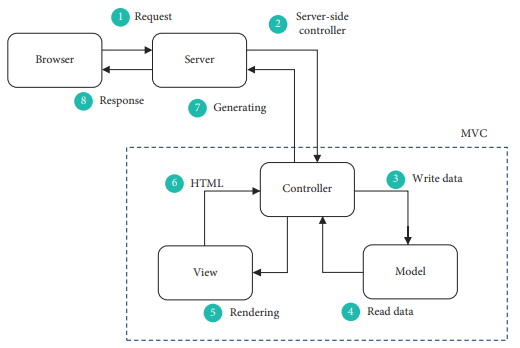
\includegraphics[width=\textwidth]{img/mvc-architecture.png}
    \caption{Arsitektur pengembangan Web menggunakan MVC}
    \label{fig:mvc-architecture}
    
    \vspace{-0.2cm}
    \begin{center}
        Sumber: Jeng et al. (2021)
    \end{center}
\end{figure}

Pola arsitektur MVC dapat diterapkan menggunakan berbagai bahasa pemrograman maupun framework dalam pengembangan aplikasi Web. Penerapan pola tersebut memungkinkan pengembang memisahkan pengelolaan data, tampilan, dan alur proses aplikasi berdasarkan tanggung jawab masing-masing komponen. Salah satu framework yang menerapkan pola MVC adalah Laravel, yaitu framework berbasis PHP yang menggunakan Model, View, dan Controller sebagai komponen utama dalam struktur aplikasinya \parencite{Purbo2021}. Dalam pengembangan SIPANTAU, Laravel digunakan sebagai framework pada sisi backend, dengan penerapan komponen Model dan Controller untuk mengelola data serta proses aplikasi. Komponen View tidak termasuk dalam lingkup pengembangan pada Praktik Kerja Lapang karena pengelolaan antarmuka pengguna dilakukan pada sisi frontend.

\section{Basis Data dan MySQL}

Basis data dan sistem manajemen basis data (\textit{Database Management System}/DBMS) merupakan dua komponen utama dalam sistem informasi. DBMS berkaitan dengan pengelolaan data yang terdapat dalam basis data dan menjadi salah satu komponen yang mendukung pengoperasian sistem informasi. Dalam pengelolaan basis data, \textit{Structured Query Language} (SQL) digunakan sebagai bahasa kueri untuk mengambil data dari basis data serta melakukan berbagai tugas pengelolaan data. SQL juga memiliki keterkaitan erat dengan DBMS karena sebagian besar DBMS modern menggunakan SQL sebagai bahasa kueri untuk mengelola data \parencite{Taipalus2021}. Dengan demikian, SQL menjadi salah satu bahasa yang digunakan dalam proses pengambilan dan pengelolaan data pada sistem manajemen basis data.

Salah satu model yang digunakan dalam pengelolaan basis data adalah model relasional. Pada model basis data relasional, data disusun dalam sekumpulan tabel yang dikelompokkan berdasarkan baris dan kolom. Tabel digunakan sebagai struktur untuk mengorganisasi data, sedangkan kolom merepresentasikan atribut dari data yang disimpan dan baris merepresentasikan entri atau rekaman data. Setiap rekaman dalam tabel dapat memiliki \textit{primary key} yang digunakan untuk mengidentifikasi rekaman secara unik. Selain itu, \textit{foreign key} dapat digunakan untuk menghubungkan tabel yang memiliki keterkaitan \parencite{Bonteanu2024}. Struktur tabel beserta hubungan antar-data tersebut digunakan untuk mengorganisasi informasi dalam basis data relasional.

MySQL merupakan salah satu sistem manajemen basis data relasional (\textit{Relational Database Management System}/RDBMS) yang bersifat \textit{open-source} dan memiliki basis pengguna yang luas. MySQL juga banyak digunakan dalam pengembangan aplikasi web serta menyediakan berbagai kemampuan untuk mendukung pengelolaan basis data, seperti replikasi, \textit{full-text search}, dan dukungan terhadap berbagai \textit{storage engine} \parencite{Bonteanu2024}. Dalam penerapannya sebagai basis data relasional, MySQL menyusun data dalam bentuk tabel yang memiliki kolom sebagai bagian dari struktur data \parencite{Gyrdi2021}. Győrödi et al. juga membedakan MySQL sebagai basis data relasional dengan \textit{document-based MySQL} sebagai pendekatan basis data non-relasional.

\section{Identification, Authentication, dan Role-Based Access Control Authorization}

Dalam sistem informasi, proses pengendalian akses terhadap sumber daya diawali dengan \textit{identification}, yaitu proses menghubungkan seseorang dengan identitas tertentu dari sejumlah identitas yang tersedia. Proses tersebut kemudian dilanjutkan dengan \textit{authentication} dan \textit{authorization}. \textit{Identification} berfungsi untuk menentukan identitas yang digunakan oleh pengguna dalam sistem dan \textit{Authentication} yang merupakan tahap berikutnya memastikan identitas yang diberikan memang milik orang tersebut \parencite{Bucko2023}.

\textit{Authentication} merupakan proses untuk menentukan apakah pengguna atau proses merupakan entitas yang sesuai dengan identitas yang diklaimnya. Proses ini memastikan bahwa entitas yang melakukan komunikasi dengan sistem merupakan entitas yang sah. Kredensial yang digunakan dalam \textit{authentication} dapat berupa sesuatu yang diketahui pengguna, seperti PIN atau kata sandi, sesuatu yang dimiliki pengguna, seperti kartu pintar atau sertifikat digital, serta karakteristik pengguna, seperti biometrik. Dengan demikian, \textit{authentication} berperan dalam memvalidasi pengguna sebelum sistem memberikan akses terhadap sumber daya yang dilindungi \parencite{Bucko2023}.

Setelah identitas pengguna berhasil diverifikasi melalui \textit{authentication}, sistem perlu menentukan hak akses yang dimiliki oleh pengguna tersebut. Proses ini disebut \textit{authorization}, yaitu teknik keamanan yang digunakan untuk menentukan privilege pengguna atau kesesuaiannya dalam melakukan tugas tertentu pada sistem. \textit{Authorization} merupakan tahapan setelah \textit{identification} dan \textit{authentication} dalam proses pemberian akses. Berbeda dengan \textit{authentication} yang menghasilkan keputusan mengenai keabsahan identitas, \textit{authorization} menentukan batasan akses pengguna terhadap berbagai sumber daya sistem sesuai dengan hak yang dimilikinya \parencite{Bucko2023}.

Salah satu strategi yang dapat digunakan dalam \textit{authorization} adalah \textit{Role-Based Access Control} (RBAC). Pada RBAC, hak akses tidak diberikan secara langsung kepada setiap pengguna, tetapi dikaitkan dengan role yang dimiliki pengguna. Role tersebut memiliki sekumpulan permission yang menentukan tindakan atau sumber daya yang dapat diakses. Kamboj et al. menjelaskan bahwa struktur RBAC terdiri atas tiga entitas utama, yaitu \textit{users}, \textit{roles}, dan \textit{permissions}, yang dihubungkan melalui hubungan \textit{user-role assignment} dan \textit{role-permission assignment}. Dengan pendekatan tersebut, permission dapat diberikan kepada pengguna berdasarkan role yang sesuai dengan tugas atau tanggung jawabnya \parencite{Kamboj2021}.

Penerapan access control tersebut juga relevan pada aplikasi berbasis web. Le et al. menjelaskan bahwa access control merupakan mekanisme keamanan untuk menentukan pengguna yang dapat mengakses suatu sumber daya serta tindakan yang dapat dilakukan terhadap sumber daya tersebut. Dalam aplikasi web, sumber daya dapat berupa halaman server, halaman client, gambar, maupun berkas lainnya, sedangkan permission dapat merepresentasikan kemampuan untuk mengakses suatu sumber daya melalui metode HTTP tertentu, seperti GET dan POST. Oleh karena itu, penerapan RBAC pada aplikasi web dapat digunakan untuk menentukan sumber daya dan operasi yang dapat dilakukan berdasarkan role pengguna \parencite{Le2022}.

\section{Integrasi Model Prediksi pada Aplikasi Berbasis Web}

Model machine learning yang telah dikembangkan dapat diintegrasikan ke dalam aplikasi berbasis web untuk menyediakan fungsi prediksi yang dapat digunakan secara langsung oleh pengguna. \cite{Alboaneen2022} misalnya, mengembangkan sistem prediksi berbasis web yang menggunakan model machine learning untuk memprediksi performa akademik mahasiswa. Sistem tersebut tersedia pada online server sehingga dapat digunakan oleh tutor. Hal ini menunjukkan bahwa aplikasi berbasis web dapat digunakan sebagai media untuk menyediakan hasil prediksi dari model machine learning kepada pengguna.

Dalam proses integrasi, model prediksi yang telah tersedia dapat digunakan sebagai komponen inference pada aplikasi tanpa harus melakukan pengembangan model dari awal. \cite{Goh2023} menjelaskan bahwa penggunaan kembali (reuse) model pre-trained merupakan salah satu pendekatan yang dapat digunakan dalam pengembangan aplikasi deep learning berbasis web. Pendekatan tersebut memungkinkan model yang telah dilatih sebelumnya untuk digunakan kembali dalam aplikasi sehingga proses pengembangan dapat difokuskan pada integrasi model dengan lingkungan aplikasi dan penyediaan antarmuka bagi pengguna.

Implementasi integrasi tersebut pada dasarnya melibatkan alur antara masukan pengguna, model prediksi, dan keluaran sistem. \cite{Mohammed2022} menunjukkan proses serupa ketika mengimplementasikan model prediksi yang sebelumnya dikembangkan dalam lingkungan R ke dalam aplikasi berbasis web. Setelah model dikonversi ke format yang kompatibel dengan JavaScript, pengguna dapat memasukkan data melalui halaman web, kemudian data tersebut diteruskan ke model untuk menghasilkan prediksi. Hasil prediksi selanjutnya dikembalikan dan ditampilkan pada halaman web.

Selain integrasi antara aplikasi dan model, kesesuaian format data juga menjadi bagian penting dalam proses inference. \cite{Mohammed2022} menunjukkan bahwa model yang dikembangkan menggunakan suatu lingkungan pemrograman belum tentu dapat langsung digunakan pada lingkungan aplikasi web sehingga diperlukan penyesuaian atau konversi agar model dapat dijalankan pada lingkungan target. Dalam penelitian tersebut, model yang dikembangkan menggunakan R dikonversi ke format yang kompatibel dengan JavaScript sebelum digunakan pada aplikasi web. Hal ini menunjukkan bahwa proses integrasi tidak hanya mencakup pemanggilan model, tetapi juga memastikan bahwa data masukan dan keluaran memiliki format yang sesuai dengan kebutuhan model dan aplikasi.

Pendekatan tersebut juga diterapkan pada EarthAIHub oleh \cite{Sit2023}, yang menyediakan platform berbasis web untuk menggunakan pre-trained deep learning models. Platform tersebut menggunakan abstraction layer untuk menjembatani aplikasi dengan model sehingga model dapat digunakan melalui platform yang sama. Konfigurasi model digunakan untuk mendefinisikan format masukan dan keluaran serta proses preprocessing dan postprocessing. Dengan demikian, integrasi model pada aplikasi dapat dipandang sebagai suatu alur yang mencakup penerimaan data masukan, penyesuaian data melalui preprocessing, proses inference menggunakan model, serta pengolahan keluaran sebelum ditampilkan kepada pengguna.

Berdasarkan pendekatan tersebut, integrasi model Chronos-v2 pada aplikasi SIPANTAU dilakukan dengan memanfaatkan model dan pipeline yang telah tersedia sebagai komponen prediksi. Aplikasi bertugas menyediakan antarmuka bagi pengguna untuk memasukkan data, meneruskan data tersebut ke komponen pipeline sesuai format yang dibutuhkan, menjalankan proses inference, serta mengolah hasil prediksi agar dapat ditampilkan kembali melalui antarmuka aplikasi. Dengan pendekatan ini, proses pengembangan SIPANTAU berfokus pada integrasi model yang telah tersedia ke dalam sistem aplikasi, bukan pada pembangunan dan pelatihan ulang model prediksi.

% \section{Dolor}
% \label{subsec:label}

% Curabitur vel tellus ligula. In consequat quam enim, sit amet
% ullamcorper est elementum nec. Vestibulum mattis congue
% tincidunt. Duis elementum erat ac varius rutrum. Proin sagittis, neque
% scelerisque sodales pharetra, nulla lacus ornare est, et cursus urna
% ex ut turpis. Morbi auctor, erat vitae semper cursus, nibh ipsum
% tristique lorem, maximus ultrices massa neque eu risus. Interdum et
% malesuada fames ac ante ipsum primis in faucibus.


% \section{Sit}
% \label{subsec:label}

% Curabitur vel tellus ligula. In consequat quam enim, sit amet
% ullamcorper est elementum nec. Vestibulum mattis congue
% tincidunt. Duis elementum erat ac varius rutrum. Proin sagittis, neque
% scelerisque sodales pharetra, nulla lacus ornare est, et cursus urna
% ex ut turpis. Morbi auctor, erat vitae semper cursus, nibh ipsum
% tristique lorem, maximus ultrices massa neque eu risus. Interdum et
% malesuada fames ac ante ipsum primis in faucibus.

% \begin{itemize}
% \item Dolor
% \item Sit
% \item Amet
% \end{itemize}


% \section{Penarikan Kesimpulan}
% \label{subsec:label}

% Phasellus porttitor purus \textcite{warn} vitae finibus laoreet. Class
% aptent taciti sociosqu ad litora torquent per conubia nostra, per
% inceptos himenaeos. Lorem ipsum dolor sit amet, consectetur adipiscing
% elit. Nunc tempus sed purus sit amet porta. Sed volutpat est ac arcu
% porttitor, non pharetra tortor pharetra. Phasellus vitae dictum
% elit. Curabitur elementum consequat elementum. Integer in vulputate
% metus. Aliquam erat volutpat. Phasellus vitae convallis orci. Etiam ac
% metus tristique, viverra metus a, mattis lectus. Aenean vel vestibulum
% augue.

% \section{Jadwal penelitian}
% \label{subsec:label}

%%%%%%%%%%%%%%%%%%%%%%%%%%%%%%%%%%%%%%%%%%%%%%%%%%%%%%%%%%%%%%%%%%%%%%%
% BAB 3
%%%%%%%%%%%%%%%%%%%%%%%%%%%%%%%%%%%%%%%%%%%%%%%%%%%%%%%%%%%%%%%%%%%%%%%

\mychapter{4}{BAB 4 METODOLOGI}

\section{Tahapan Pelaksanaan}

Pelaksanaan Praktik Kerja Lapang (PKL) pada pengembangan aplikasi web SIPANTAU dilakukan dengan melanjutkan pengembangan sistem yang telah berjalan sebelumnya. Pada awal pelaksanaan PKL, sistem telah memiliki antarmuka \textit{frontend} yang menggunakan data \textit{dummy}, rancangan awal basis data, serta kebutuhan utama sistem yang meliputi pengelolaan data komoditas, prediksi harga komoditas untuk tiga hari ke depan pada pasar tertentu, dan penerapan autentikasi serta otorisasi berdasarkan peran pengguna. Selain itu, Laravel telah ditetapkan sebagai \textit{framework} yang digunakan pada sisi \textit{backend}. Kondisi tersebut menjadi dasar dalam melakukan analisis terhadap sistem yang telah tersedia serta menentukan komponen yang perlu dirancang dan dikembangkan selama pelaksanaan PKL. Dengan demikian, kegiatan pengembangan difokuskan pada basis data dan \textit{backend}, mekanisme autentikasi dan otorisasi, integrasi layanan model prediksi, serta \textit{deployment} aplikasi.

Tahapan pelaksanaan diawali dengan analisis kondisi dan kebutuhan sistem yang telah ada untuk memahami kebutuhan fungsional serta hubungan antara \textit{frontend}, \textit{backend}, basis data, dan layanan model prediksi. Berdasarkan hasil analisis tersebut, dilakukan perancangan basis data dan arsitektur \textit{backend}, perancangan autentikasi dan otorisasi, perancangan integrasi layanan model prediksi, serta perancangan \textit{deployment} aplikasi. Setiap rancangan kemudian menjadi dasar bagi tahap implementasi masing-masing komponen. Implementasi dilakukan secara bertahap mulai dari basis data dan \textit{backend}, kemudian autentikasi dan otorisasi, integrasi layanan model prediksi, hingga \textit{deployment} aplikasi.

\begin{figure}[H]
    \centering
    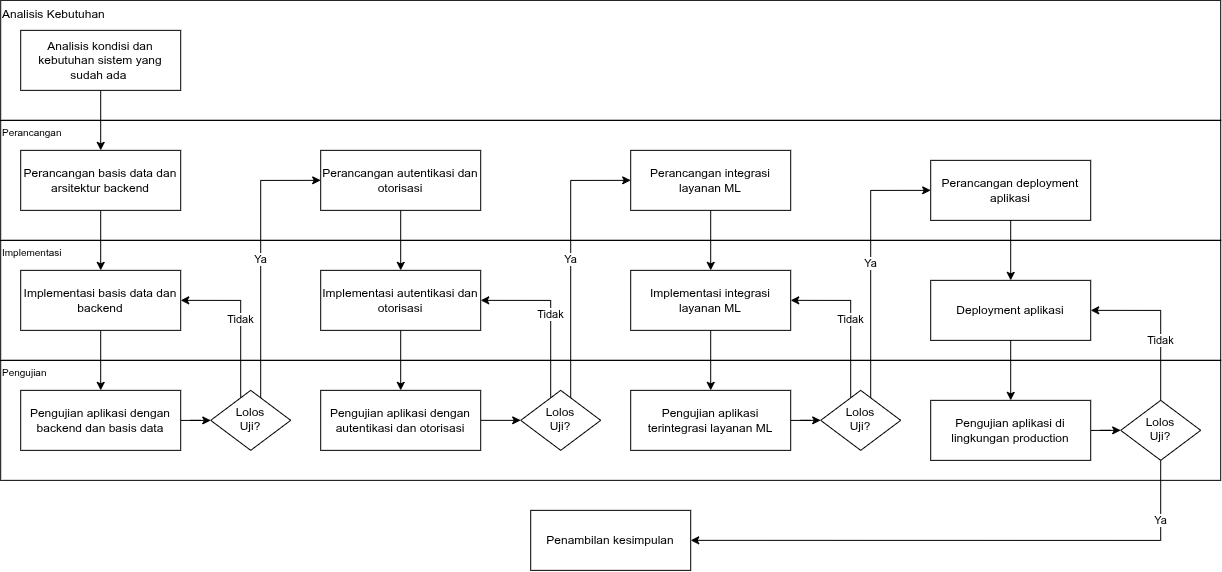
\includegraphics[width=\textwidth]{img/tahapan-pelaksanaan.png}
    \caption{Tahapan Pelaksanaan PKL}
    \label{fig:tahapan-pelaksanaan}
\end{figure}

Setiap hasil implementasi diuji sebelum proses dilanjutkan ke tahap berikutnya. Apabila hasil pengujian belum memenuhi kebutuhan yang ditetapkan, dilakukan penyesuaian terhadap implementasi terkait dan pengujian dilakukan kembali hingga hasil yang diperoleh sesuai dengan kebutuhan sistem. Setelah seluruh komponen aplikasi berhasil melalui pengujian pada lingkungan pengembangan, dilakukan \textit{deployment} ke lingkungan \textit{production} yang telah dirancang. Aplikasi yang telah di-\textit{deploy} kemudian diuji kembali pada lingkungan \textit{production} untuk memastikan sistem dapat berjalan pada lingkungan operasional. Tahapan pelaksanaan secara keseluruhan ditunjukkan pada Gambar~\ref{fig:tahapan-pelaksanaan}.

\section{Spesifikasi Hardware dan Software}

Pengembangan dan \textit{deployment} aplikasi web SIPANTAU dilakukan pada lingkungan komputasi berbasis \textit{Virtual Private Server} (VPS). Infrastruktur tersebut menggunakan virtualisasi Xen dengan arsitektur x86-64 dan sistem operasi Ubuntu 24.04.4 LTS. Server menyediakan 8 \textit{virtual CPU} dengan prosesor Intel Xeon E5-2620 v4 berfrekuensi 2.10 GHz serta memori sebesar 4 GB. Spesifikasi perangkat keras tersebut digunakan sebagai lingkungan untuk menjalankan komponen aplikasi selama proses pengembangan dan \textit{deployment}. Rincian spesifikasi perangkat keras yang digunakan ditunjukkan pada Tabel~\ref{tab:spesifikasi-hardware}.

\begin{table}[H]
    \centering
    \caption{Spesifikasi Perangkat Keras}
    \label{tab:spesifikasi-hardware}
    \begin{tabular}{|l|l|}
        \hline
        \textbf{Komponen} & \textbf{Spesifikasi} \\ \hline
        Jenis perangkat & Virtual Private Server (VPS) \\ \hline
        Virtualisasi & Xen \\ \hline
        Prosesor & Intel Xeon E5-2620 v4 @ 2.10 GHz \\ \hline
        CPU & 8 vCPU \\ \hline
        Memori & 4 GB \\ \hline
        Arsitektur & x86-64 \\ \hline
        Sistem operasi & Ubuntu 24.04.4 LTS \\ \hline
    \end{tabular}
\end{table}

Perangkat lunak yang digunakan terdiri atas komponen untuk pengembangan \textit{backend}, pengelolaan basis data, pengembangan \textit{frontend}, penyajian aplikasi, serta pengelolaan lingkungan aplikasi. Laravel 12.49.0 digunakan sebagai \textit{framework backend} dengan PHP 8.4.21 sebagai lingkungan eksekusinya, sedangkan Composer 2.9.8 digunakan untuk mengelola dependensi PHP. Basis data aplikasi menggunakan MySQL 8.4.8, sementara sisi \textit{frontend} menggunakan Node.js 20.20.2 dan NPM 10.8.2 sebagai lingkungan dan pengelola paket JavaScript. Docker 29.4.0 digunakan untuk menjalankan komponen aplikasi dalam lingkungan \textit{container}, Nginx 1.29.8 digunakan sebagai \textit{web server}, dan Git 2.43.0 digunakan untuk pengelolaan versi kode sumber. Rincian perangkat lunak yang digunakan ditunjukkan pada Tabel~\ref{tab:spesifikasi-software}.

\begin{table}[H]
    \centering
    \caption{Spesifikasi Perangkat Lunak}
    \label{tab:spesifikasi-software}
    \begin{tabular}{|l|l|l|}
        \hline
        \textbf{Perangkat Lunak} & \textbf{Versi} & \textbf{Fungsi} \\ \hline
        Ubuntu & 24.04.4 LTS & Sistem operasi \\ \hline
        PHP & 8.4.21 & Runtime backend \\ \hline
        Laravel & 12.49.0 & Framework backend \\ \hline
        Composer & 2.9.8 & Pengelola dependensi PHP \\ \hline
        MySQL & 8.4.8 & Sistem manajemen basis data \\ \hline
        Node.js & 20.20.2 & Runtime JavaScript frontend \\ \hline
        NPM & 10.8.2 & Pengelola paket frontend \\ \hline
        Nginx & 1.29.8 & Web server \\ \hline
        Docker & 29.4.0 & Pengelola container \\ \hline
        Git & 2.43.0 & Version control \\ \hline
    \end{tabular}
\end{table}

\section{Metode Perancangan}

Metode perancangan digunakan sebagai dasar dalam menentukan struktur dan mekanisme kerja komponen aplikasi yang akan dikembangkan sebelum dilakukan implementasi. Perancangan dilakukan berdasarkan kondisi awal sistem, kebutuhan aplikasi, serta keterkaitan antara komponen yang telah tersedia dengan komponen yang perlu dikembangkan. Proses perancangan mencakup basis data dan arsitektur \textit{backend}, mekanisme \textit{authentication} dan \textit{authorization}, integrasi layanan model prediksi, serta \textit{deployment} aplikasi. Setiap rancangan disusun untuk menghasilkan spesifikasi teknis yang dapat digunakan sebagai acuan pada tahap implementasi.

\subsection{Analisis Kondisi dan Kebutuhan Sistem}

Analisis kondisi dan kebutuhan sistem dilakukan untuk memahami keadaan awal aplikasi serta menentukan fungsi yang perlu disediakan oleh komponen yang dikembangkan. Pada awal pelaksanaan PKL, aplikasi telah memiliki \textit{frontend} yang menggunakan data \textit{dummy}, rancangan awal basis data, dan kebutuhan utama sistem. Kebutuhan tersebut mencakup pengelolaan data komoditas, prediksi harga komoditas untuk tiga hari ke depan pada pasar tertentu, serta penerapan \textit{authentication} dan \textit{authorization} berdasarkan peran pengguna. Selain kebutuhan tersebut, Laravel telah ditetapkan sebagai \textit{framework} yang digunakan untuk membangun sisi \textit{backend}. Hasil analisis terhadap kondisi dan kebutuhan tersebut kemudian digunakan sebagai dasar untuk menentukan rancangan basis data, arsitektur \textit{backend}, mekanisme pengendalian akses, integrasi layanan model prediksi, dan kebutuhan \textit{deployment}.

\subsection{Perancangan Basis Data dan Arsitektur Backend}

Perancangan basis data dilakukan dengan menyesuaikan struktur penyimpanan data terhadap kebutuhan fungsional aplikasi. Proses perancangan mencakup penentuan entitas yang diperlukan, atribut pada setiap entitas, serta hubungan antarentitas yang digunakan dalam pengelolaan data aplikasi. Hasil perancangan basis data digunakan sebagai acuan dalam menentukan struktur tabel dan relasi yang akan diimplementasikan pada sistem manajemen basis data. Rancangan basis data kemudian diselaraskan dengan kebutuhan \textit{backend} agar data yang diperlukan oleh setiap fungsi aplikasi dapat disediakan secara terstruktur.

Perancangan arsitektur \textit{backend} dilakukan untuk menentukan pembagian komponen dan aliran data antara \textit{frontend}, \textit{backend}, basis data, dan layanan pendukung lainnya. Laravel digunakan sebagai dasar perancangan sisi \textit{backend}, dengan komponen aplikasi disusun berdasarkan tanggung jawab masing-masing dalam menerima permintaan, memproses data, berinteraksi dengan basis data, dan menghasilkan respons kepada \textit{frontend}. Perancangan juga mencakup penentuan \textit{route} dan mekanisme komunikasi yang diperlukan agar fungsi pengelolaan data dan fungsi lainnya dapat diakses oleh \textit{frontend}. Rancangan tersebut selanjutnya digunakan sebagai acuan pada tahap implementasi \textit{backend} dan basis data.

\subsection{Perancangan Authentication dan Authorization}

Perancangan \textit{authentication} dan \textit{authorization} dilakukan untuk memastikan bahwa akses terhadap fungsi dan sumber daya aplikasi diberikan sesuai dengan identitas serta peran pengguna. Mekanisme \textit{authentication} dirancang untuk melakukan verifikasi terhadap pengguna sebelum pengguna dapat mengakses fungsi yang memerlukan autentikasi. Setelah pengguna berhasil diautentikasi, sistem menggunakan informasi peran pengguna sebagai dasar dalam menentukan hak akses terhadap sumber daya dan fungsi tertentu. Dengan demikian, pengguna dengan peran yang berbeda dapat memiliki tingkat akses yang berbeda sesuai dengan kebutuhan sistem.

Perancangan hak akses dilakukan menggunakan pendekatan berbasis peran, dengan setiap peran memiliki kumpulan izin terhadap fungsi atau sumber daya tertentu. Hubungan antara pengguna, peran, dan hak akses ditentukan terlebih dahulu agar mekanisme pengendalian akses dapat diterapkan secara konsisten pada \textit{backend}. Rancangan tersebut kemudian menjadi dasar dalam menentukan mekanisme pemeriksaan hak akses pada setiap fungsi atau \textit{endpoint} yang membutuhkan pembatasan akses. Hasil perancangan ini selanjutnya digunakan sebagai acuan dalam implementasi \textit{authentication} dan \textit{authorization}.

\subsection{Perancangan Integrasi Layanan Model Prediksi}

Perancangan integrasi layanan model prediksi dilakukan untuk menentukan mekanisme pertukaran data antara aplikasi web dengan model prediksi yang telah tersedia. Model prediksi tidak dikembangkan atau dilatih kembali dalam pelaksanaan PKL, melainkan digunakan sebagai komponen yang diintegrasikan ke dalam aplikasi untuk menghasilkan prediksi harga komoditas. Perancangan difokuskan pada aliran data mulai dari permintaan prediksi oleh pengguna, pengambilan data historis yang diperlukan, persiapan data, pemanggilan model, hingga pengembalian hasil prediksi kepada \textit{frontend}. Alur tersebut dirancang agar proses prediksi dapat dijalankan melalui aplikasi tanpa mengharuskan pengguna berinteraksi secara langsung dengan model.

Data yang digunakan sebagai masukan model perlu dipersiapkan dalam format yang sesuai dengan kebutuhan layanan prediksi. Oleh karena itu, rancangan integrasi mencakup proses pengambilan data historis komoditas dari basis data, penyesuaian struktur data, pengiriman data kepada pipeline model prediksi, serta pengolahan hasil prediksi sebelum diberikan kepada \textit{frontend}. Pipeline Chronos-v2 digunakan sebagai komponen prediksi dalam rancangan tersebut. Secara umum, aliran integrasi dirancang dari \textit{frontend} menuju \textit{backend}, kemudian menuju pipeline model prediksi, dan hasil prediksi dikembalikan melalui \textit{backend} untuk ditampilkan kepada pengguna.

\subsection{Perancangan Deployment Aplikasi}

Perancangan \textit{deployment} dilakukan untuk menentukan konfigurasi lingkungan yang diperlukan agar aplikasi dapat dijalankan pada lingkungan \textit{production}. Perancangan mencakup pembagian komponen aplikasi ke dalam lingkungan eksekusi, konfigurasi layanan aplikasi, koneksi basis data, serta komunikasi antara \textit{frontend}, \textit{backend}, dan layanan pendukung. Penggunaan Docker dirancang untuk menyediakan lingkungan eksekusi berbasis \textit{container} bagi komponen aplikasi, sedangkan Nginx digunakan sebagai bagian dari konfigurasi penyajian aplikasi. Rancangan tersebut juga mempertimbangkan konfigurasi variabel lingkungan dan dependensi yang diperlukan oleh masing-masing komponen.

Rancangan \textit{deployment} digunakan sebagai acuan dalam proses pemasangan dan konfigurasi aplikasi pada VPS. Setelah aplikasi berhasil ditempatkan pada lingkungan \textit{production}, dilakukan pengujian untuk memastikan setiap komponen dapat berkomunikasi dan menjalankan fungsi sesuai dengan rancangan. Apabila ditemukan permasalahan pada hasil pengujian, konfigurasi atau komponen \textit{deployment} disesuaikan dan proses \textit{deployment} serta pengujian dilakukan kembali. Dengan demikian, rancangan \textit{deployment} tidak hanya menentukan konfigurasi awal lingkungan \textit{production}, tetapi juga menjadi dasar dalam proses penyesuaian hingga aplikasi dapat berjalan sesuai kebutuhan.

\section{Metode Implementasi}

Metode implementasi merupakan tahapan penerapan hasil perancangan menjadi komponen aplikasi yang dapat dijalankan dan digunakan sesuai dengan kebutuhan sistem. Implementasi dilakukan secara bertahap berdasarkan rancangan basis data dan arsitektur \textit{backend}, mekanisme \textit{authentication} dan \textit{authorization}, integrasi layanan model prediksi, serta rancangan \textit{deployment}. Setiap komponen diimplementasikan sesuai dengan rancangan yang telah ditetapkan dan disesuaikan apabila ditemukan kondisi teknis yang memerlukan perubahan selama proses pengembangan. Hasil implementasi pada setiap tahapan selanjutnya digunakan sebagai dasar untuk melakukan pengujian terhadap fungsi yang telah dikembangkan.

\subsection{Implementasi Basis Data dan Backend}

Implementasi basis data dilakukan dengan merealisasikan rancangan struktur data ke dalam MySQL menggunakan mekanisme migration Laravel. Migration digunakan untuk membentuk tabel, atribut, serta relasi yang diperlukan oleh aplikasi sesuai dengan kebutuhan sistem. Selain itu, data awal yang diperlukan oleh aplikasi dimasukkan menggunakan mekanisme seeder yang tersedia pada Laravel. Struktur basis data yang telah dibuat kemudian digunakan oleh \textit{backend} sebagai sumber data dalam menjalankan fungsi pengelolaan data aplikasi.

Implementasi \textit{backend} dilakukan menggunakan Laravel dengan menerapkan pola \textit{Model} dan \textit{Controller} untuk menangani interaksi antara aplikasi dan basis data. Controller digunakan untuk menerima permintaan dari \textit{frontend}, melakukan pemrosesan yang diperlukan, serta menghasilkan respons melalui \textit{API}. Fungsi pengelolaan data diimplementasikan melalui beberapa Controller yang menangani data komoditas, pasar, panen, harga pasar harian, harga petani harian, dan ketersediaan harian. Data yang diperoleh dari basis data kemudian disusun menjadi respons API menggunakan komponen \textit{Resource} pada Laravel sebelum diteruskan kepada \textit{frontend}.

\subsection{Implementasi Authentication dan Authorization}

Implementasi \textit{authentication} dilakukan melalui \textit{endpoint} yang disediakan oleh AuthController. Proses tersebut mencakup pendaftaran pengguna, proses \textit{login}, pengelolaan sesi autentikasi, dan \textit{logout}. Laravel Sanctum digunakan sebagai mekanisme autentikasi berbasis token untuk mengidentifikasi pengguna yang melakukan permintaan terhadap layanan \textit{backend}. Token autentikasi kemudian digunakan dalam permintaan yang membutuhkan identitas pengguna, sehingga sistem dapat membedakan permintaan yang telah terautentikasi dengan permintaan yang tidak memiliki autentikasi yang valid.

Implementasi \textit{authorization} dilakukan dengan menerapkan pembatasan akses berdasarkan peran dan izin pengguna menggunakan paket \textit{Spatie Laravel Permission}. Peran dan izin disimpan pada basis data melalui tabel yang disediakan oleh paket tersebut, kemudian digunakan untuk menentukan fungsi yang dapat diakses oleh pengguna. Mekanisme pembatasan akses diterapkan pada \textit{endpoint} yang memerlukan hak akses tertentu sehingga pengguna hanya dapat menjalankan operasi sesuai dengan peran dan izin yang dimilikinya. Selain itu, informasi aktivitas pengguna dicatat melalui ActivityLogger pada fungsi tertentu, termasuk ketika pengguna mengakses fungsi prediksi.

\subsection{Implementasi Integrasi Layanan Model Prediksi}

Implementasi integrasi layanan model prediksi dilakukan dengan menghubungkan \textit{backend} Laravel dengan layanan model prediksi yang dijalankan secara terpisah. Ketika pengguna meminta prediksi berdasarkan komoditas dan pasar tertentu, \textit{frontend} mengirimkan pasar\_id dan komoditas\_id kepada \textit{backend}. Parameter tersebut terlebih dahulu divalidasi untuk memastikan bahwa pasar dan komoditas yang diminta tersedia pada basis data. Selanjutnya, \textit{backend} mengambil data harga pasar harian dan data pendukung berupa ketersediaan, kebutuhan, serta neraca harian berdasarkan komoditas dan pasar yang dipilih. Data yang digunakan dibatasi pada sepuluh data historis terakhir dan diurutkan kembali berdasarkan urutan waktu sebelum digunakan sebagai masukan model. Alur integrasi layanan model prediksi secara keseluruhan ditunjukkan pada Gambar \ref{fig:alur-prediksi}.

\begin{figure}[H]
    \centering
    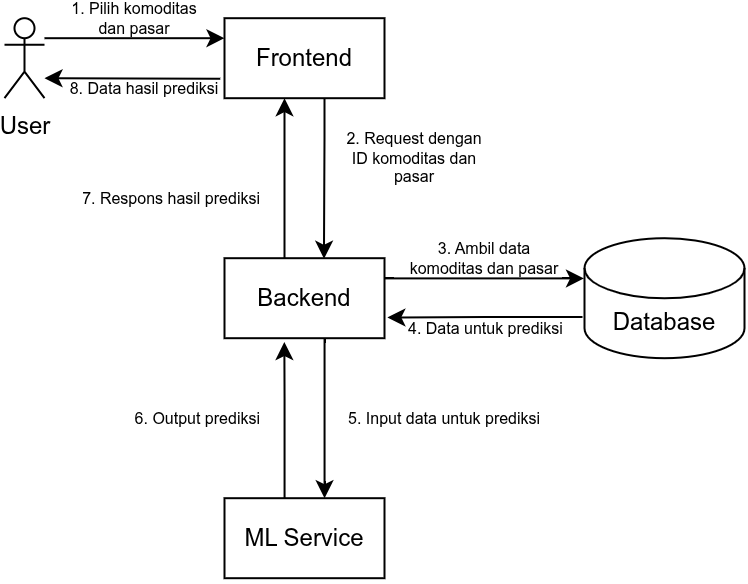
\includegraphics[width=0.8\textwidth]{img/alur-prediksi.png}
    \caption{Alur integrasi layanan model prediksi}
    \label{fig:alur-prediksi}
\end{figure}

Data historis yang telah diperoleh kemudian disusun menjadi struktur masukan yang terdiri atas nilai harga pasar, ketersediaan harian, kebutuhan harian, dan neraca harian. Setiap nilai dikonversi menjadi tipe numerik sebelum dikirimkan kepada layanan model prediksi. \textit{Backend} kemudian melakukan permintaan HTTP \textit{POST} ke layanan \textit{machine learning} pada /predict melalui jaringan internal Docker dengan alamat layanan ml-service:8001. Data tersebut dikirimkan dalam parameter data sebagai masukan untuk proses prediksi.

Layanan model prediksi diimplementasikan menggunakan FastAPI dan menyediakan \textit{endpoint} POST /predict untuk menerima data dari \textit{backend}. Data masukan dikonversi menjadi array numerik menggunakan NumPy, kemudian dilakukan transformasi dimensi agar sesuai dengan struktur masukan yang dibutuhkan oleh pipeline model. Pipeline Chronos-2 yang digunakan pada layanan tersebut dimuat menggunakan model autogluon/chronos2-small, dengan pemilihan perangkat komputasi GPU apabila tersedia dan CPU apabila GPU tidak tersedia.

Pipeline model kemudian dijalankan dengan panjang prediksi sebanyak tiga periode. Hasil prediksi yang diperoleh diproses untuk memperoleh nilai prediksi yang digunakan oleh aplikasi, kemudian dikembalikan oleh layanan model dalam bentuk respons JSON dengan atribut prediksi. \textit{Backend} Laravel menerima respons tersebut dan memetakan tiga nilai prediksi menjadi prediksi untuk hari pertama, hari kedua, dan hari ketiga. Hasil tersebut kemudian digabungkan dengan informasi tanggal dan harga pasar historis yang relevan sebelum dikembalikan kepada \textit{frontend} melalui respons API.

\subsection{Deployment Aplikasi}

Deployment aplikasi dilakukan pada VPS dengan menggunakan Docker untuk menjalankan komponen aplikasi dalam beberapa \textit{container}. Lingkungan \textit{production} terdiri atas \textit{container} backend, frontend, ml-service, dan nginx. Container backend digunakan untuk menjalankan aplikasi Laravel, sedangkan frontend menjalankan aplikasi sisi \textit{frontend}. Layanan model prediksi dijalankan pada ml-service, sementara Nginx digunakan untuk menerima akses dari luar dan meneruskan permintaan kepada komponen aplikasi yang sesuai.

Setiap komponen dihubungkan melalui jaringan Docker sipantau-network sehingga \textit{backend} dapat berkomunikasi dengan layanan model prediksi menggunakan nama layanan ml-service. Container backend, ml-service, dan frontend dikonfigurasi dengan restart unless-stopped agar layanan dapat dijalankan kembali secara otomatis apabila container berhenti dan Docker daemon tetap berjalan. Nginx mengekspos port 80 dan 443 untuk menyediakan akses HTTP dan HTTPS dari luar lingkungan Docker. Konfigurasi tersebut digunakan sebagai dasar dalam menjalankan aplikasi pada lingkungan \textit{production}.

\section{Metode Pengujian}

Metode pengujian digunakan untuk memastikan bahwa komponen aplikasi yang telah diimplementasikan dapat berjalan sesuai dengan kebutuhan dan rancangan sistem. Pengujian dilakukan secara bertahap pada setiap komponen dan dilanjutkan dengan pengujian setelah komponen tersebut terintegrasi dengan \textit{frontend}. Pengujian dilakukan terhadap basis data dan \textit{backend}, mekanisme \textit{authentication} dan \textit{authorization}, integrasi layanan model prediksi, serta aplikasi pada lingkungan \textit{production}. Pada pengujian tingkat layanan, permintaan dilakukan secara langsung terhadap \textit{endpoint} menggunakan Postman atau perintah \texttt{curl}, sedangkan pengujian integrasi dilakukan melalui antarmuka aplikasi untuk memastikan alur penggunaan oleh pengguna dapat berjalan dengan baik. Hasil dari setiap pengujian kemudian dibandingkan dengan kondisi atau keluaran yang diharapkan untuk menentukan kesesuaian implementasi terhadap kebutuhan sistem.

\subsection{Pengujian Basis Data dan Backend}

Pengujian basis data dan \textit{backend} dilakukan untuk memastikan bahwa fungsi pengelolaan data dan \textit{endpoint} API dapat menerima permintaan, memproses data, serta menghasilkan respons sesuai dengan kebutuhan sistem. Pengujian dilakukan menggunakan Postman terhadap setiap \textit{endpoint} yang disediakan oleh \textit{backend}, termasuk \textit{endpoint} untuk pengelolaan data aplikasi. Pengujian dilakukan dengan memberikan permintaan dan parameter yang sesuai dengan fungsi masing-masing \textit{endpoint}, kemudian memeriksa respons yang dihasilkan serta perubahan data pada basis data apabila operasi tersebut melakukan penyimpanan atau perubahan data. Setelah \textit{backend} diintegrasikan dengan \textit{frontend}, pengujian kembali dilakukan melalui antarmuka aplikasi untuk memastikan bahwa permintaan dari \textit{frontend} dapat diproses oleh \textit{backend} dan hasilnya dapat digunakan oleh aplikasi. Dengan demikian, pengujian tidak hanya memeriksa fungsi API secara langsung, tetapi juga memastikan keterhubungan antara \textit{frontend}, \textit{backend}, dan basis data. Ringkasan aspek pengujian, metode yang digunakan, dan hasil yang diharapkan ditunjukkan pada Tabel \ref{tab:pengujian-backend}.

\begin{longtable}{|p{3.2cm}|p{4.0cm}|p{4.0cm}|}
    \caption{Ringkasan pengujian basis data dan backend}
    \label{tab:pengujian-backend} \\
    \hline
    \textbf{Aspek Pengujian} & \textbf{Metode Pengujian} & \textbf{Hasil yang Diharapkan} \\
    \hline
    \endfirsthead

    \hline
    \textbf{Aspek Pengujian} & \textbf{Metode Pengujian} & \textbf{Hasil yang Diharapkan} \\
    \hline
    \endhead

    Endpoint API &
    Mengirimkan permintaan pada setiap endpoint menggunakan Postman &
    Endpoint dapat menerima dan memproses permintaan serta menghasilkan respons sesuai fungsi. \\
    \hline

    \hline
    Pengelolaan data &
    Melakukan operasi penambahan, pembacaan, perubahan, dan penghapusan data sesuai fungsi endpoint &
    Data pada basis data berubah sesuai dengan operasi yang dilakukan. \\
    \hline
    Integrasi frontend--backend &
    Menjalankan fungsi aplikasi melalui frontend setelah backend terintegrasi &
    Permintaan dari frontend dapat diproses oleh backend dan hasilnya dapat digunakan oleh aplikasi. \\
    \hline
\end{longtable}

\subsection{Pengujian Authentication dan Authorization}

Pengujian \textit{authentication} dan \textit{authorization} dilakukan untuk memastikan bahwa mekanisme akses pengguna berjalan sesuai dengan peran yang dimiliki. Pengujian diawali dengan membuat beberapa akun pengguna dengan peran yang berbeda, kemudian melakukan pengujian terhadap fungsi yang seharusnya dapat diakses maupun tidak dapat diakses oleh masing-masing peran. Pengujian dilakukan menggunakan Postman dengan mengirimkan permintaan menggunakan akun dari setiap peran dan mengamati respons yang diberikan oleh \textit{backend}. Setelah mekanisme tersebut diintegrasikan dengan \textit{frontend}, pengujian dilanjutkan melalui beberapa skenario penggunaan untuk memastikan bahwa pengguna dapat menjalankan fungsi yang menjadi hak aksesnya dan tidak dapat menjalankan fungsi yang berada di luar hak akses tersebut. Hasil pengujian digunakan untuk memastikan kesesuaian antara peran pengguna dan hak akses terhadap fungsi aplikasi. Rincian aspek pengujian, metode pengujian, dan hasil yang diharapkan dirangkum pada Tabel \ref{tab:pengujian-auth}.

\begin{longtable}{|p{3.2cm}|p{4.0cm}|p{4.0cm}|}
    \caption{Ringkasan pengujian authentication dan authorization}
    \label{tab:pengujian-auth} \\
    \hline
    \textbf{Aspek Pengujian} & \textbf{Metode Pengujian} & \textbf{Hasil yang Diharapkan} \\
    \hline
    \endfirsthead
    
    \hline
    \textbf{Aspek Pengujian} & \textbf{Metode Pengujian} & \textbf{Hasil yang Diharapkan} \\
    \hline
    \endhead
    
    Authentication &
    Melakukan proses login menggunakan akun pengguna yang telah dibuat &
    Pengguna yang memiliki kredensial yang sesuai dapat terautentikasi dan memperoleh akses ke aplikasi. \\
    \hline
    Hak akses berdasarkan peran &
    Mengirimkan permintaan menggunakan akun dengan beberapa peran yang berbeda melalui Postman &
    Setiap peran hanya dapat mengakses fungsi yang sesuai dengan hak aksesnya. \\
    \hline
    Pembatasan akses &
    Mencoba menjalankan fungsi yang tidak menjadi hak akses pengguna &
    Permintaan terhadap fungsi yang tidak diizinkan ditolak oleh sistem. \\
    \hline
    Integrasi frontend &
    Menjalankan beberapa skenario akses melalui frontend menggunakan akun dengan peran berbeda &
    Fungsi yang dapat dan tidak dapat diakses pengguna sesuai dengan peran yang dimilikinya. \\
    \hline
\end{longtable}

\subsection{Pengujian Integrasi Layanan Model Prediksi}

Pengujian integrasi layanan model prediksi dilakukan secara bertahap untuk memastikan bahwa layanan model dapat menerima data, menghasilkan prediksi, dan terhubung dengan \textit{backend} serta \textit{frontend}. Tahap pertama dilakukan secara langsung pada container \textit{ML service} menggunakan perintah \texttt{curl} untuk menguji \textit{endpoint} prediksi secara terpisah dari \textit{backend}. Pengujian ini dilakukan untuk memastikan bahwa layanan FastAPI dapat menerima data masukan dan mengembalikan hasil prediksi melalui \textit{endpoint} yang disediakan. Tahap kedua dilakukan terhadap \textit{endpoint} prediksi pada \textit{backend} menggunakan Postman untuk memastikan bahwa \textit{backend} dapat mengambil data yang diperlukan, mengirimkan data ke \textit{ML service}, menerima hasil prediksi, dan mengembalikan respons kepada pemanggil API. Tahap ketiga dilakukan setelah integrasi dengan \textit{frontend} dengan menjalankan proses prediksi melalui antarmuka aplikasi untuk memastikan seluruh alur prediksi dapat berjalan secara terpadu dari masukan pengguna hingga hasil prediksi ditampilkan. Ringkasan tahapan pengujian, metode yang digunakan, dan hasil yang diharapkan ditunjukkan pada Tabel \ref{tab:pengujian-prediksi}.

\begin{longtable}{|p{3.2cm}|p{4.0cm}|p{4.0cm}|}
    \caption{Ringkasan pengujian integrasi layanan model prediksi}
    \label{tab:pengujian-prediksi} \\
    \hline
    \textbf{Tahap Pengujian} & \textbf{Metode Pengujian} & \textbf{Hasil yang Diharapkan} \\
    \hline
    \endfirsthead

    \hline
    \textbf{Tahap Pengujian} & \textbf{Metode Pengujian} & \textbf{Hasil yang Diharapkan} \\
    \hline
    \endhead

    ML service &
    Mengirimkan data masukan secara langsung ke endpoint prediksi menggunakan \texttt{curl} &
    ML service dapat menerima data dan mengembalikan hasil prediksi. \\
    \hline
    Backend--ML service &
    Mengirimkan permintaan ke endpoint prediksi backend menggunakan Postman &
    Backend dapat mengambil data historis, mengirimkannya ke ML service, menerima hasil prediksi, dan mengembalikan respons. \\
    \hline
    Integrasi frontend &
    Menjalankan proses prediksi melalui antarmuka frontend &
    Seluruh alur prediksi dari masukan pengguna hingga hasil prediksi dapat berjalan dengan baik. \\
    \hline
\end{longtable}

\subsection{Pengujian pada Lingkungan Production}

Pengujian pada lingkungan \textit{production} dilakukan setelah seluruh komponen aplikasi berhasil diimplementasikan dan dideploy untuk memastikan sistem dapat digunakan sesuai dengan konfigurasi lingkungan sebenarnya. Pengujian mencakup pemeriksaan akses melalui protokol HTTP untuk memastikan bahwa aplikasi tidak dapat digunakan melalui koneksi yang tidak memenuhi konfigurasi keamanan yang ditetapkan, serta pengujian skenario penggunaan oleh beberapa pengguna dengan peran yang berbeda. Pada setiap skenario, dilakukan pengujian terhadap fungsi yang seharusnya dapat dijalankan maupun fungsi yang seharusnya dibatasi berdasarkan peran pengguna. Selain itu, proses prediksi dilakukan melalui \textit{frontend} pada lingkungan \textit{production} untuk memastikan bahwa komunikasi antara \textit{frontend}, \textit{backend}, dan \textit{ML service} dapat berjalan pada lingkungan deployment. Hasil pengujian digunakan untuk memastikan bahwa aplikasi dapat menjalankan fungsi utama dan mekanisme akses sesuai dengan rancangan setelah diterapkan pada lingkungan \textit{production}. Ringkasan aspek pengujian, metode pengujian, dan hasil yang diharapkan pada lingkungan \textit{production} ditunjukkan pada Tabel \ref{tab:pengujian-production}.

\begin{longtable}{|p{3.2cm}|p{4.0cm}|p{4.0cm}|}
    \caption{Ringkasan pengujian pada lingkungan production}
    \label{tab:pengujian-production} \\
    \hline
    \textbf{Aspek Pengujian} & \textbf{Metode Pengujian} & \textbf{Hasil yang Diharapkan} \\
    \hline
    \endfirsthead

    \hline
    \textbf{Aspek Pengujian} & \textbf{Metode Pengujian} & \textbf{Hasil yang Diharapkan} \\
    \hline
    \endhead

    Protokol akses &
    Mencoba mengakses aplikasi melalui protokol HTTP &
    Aplikasi tidak dapat digunakan melalui koneksi HTTP sesuai konfigurasi keamanan yang diterapkan. \\
    \hline
    Hak akses pengguna &
    Menjalankan skenario penggunaan menggunakan beberapa akun dengan peran yang berbeda &
    Pengguna dapat menjalankan fungsi sesuai dengan hak akses yang dimiliki dan tidak dapat menjalankan fungsi yang dibatasi. \\
    \hline
    Proses input data &
    Melakukan input data melalui frontend pada lingkungan production &
    Data dapat dikirim dan diproses oleh sistem sesuai dengan fungsi aplikasi. \\
    \hline
    Proses prediksi &
    Menjalankan proses prediksi melalui frontend pada lingkungan production &
    Proses prediksi dapat berjalan dan hasil prediksi dapat ditampilkan kepada pengguna. \\
    \hline
\end{longtable}

% Donec vitae rutrum arcu. Aenean dictum mauris id lobortis
% vulputate. In ut pretium turpis. Nunc elit nunc, blandit et maximus
% at, maximus at orci. Aliquam a nisl pretium, eleifend odio sit amet,
% interdum augue. Donec magna elit, cursus gravida libero vitae, congue
% luctus sapien. Phasellus sit amet nisl sed nisl dictum
% porttitor. Etiam viverra lacus est, a ultrices nisi euismod ut.

% \section{Studi Literatur}
% \label{subsec:label}

% Donec vitae rutrum arcu. Aenean dictum mauris id lobortis
% vulputate. In ut pretium turpis. Nunc elit nunc, blandit et maximus
% at, maximus at orci. Aliquam a nisl pretium, eleifend odio sit amet,
% interdum augue. Donec magna elit, cursus gravida libero vitae, congue
% luctus sapien. Phasellus sit amet nisl sed nisl dictum
% porttitor. Etiam viverra lacus est, a ultrices nisi euismod ut.


% \section{Dolor}
% \label{subsec:label}

% Curabitur vel tellus ligula. In consequat quam enim, sit amet
% ullamcorper est elementum nec. Vestibulum mattis congue
% tincidunt. Duis elementum erat ac varius rutrum. Proin sagittis, neque
% scelerisque sodales pharetra, nulla lacus ornare est, et cursus urna
% ex ut turpis. Morbi auctor, erat vitae semper cursus, nibh ipsum
% tristique lorem, maximus ultrices massa neque eu risus. Interdum et
% malesuada fames ac ante ipsum primis in faucibus.


% \section{Sit}
% \label{subsec:label}

% Curabitur vel tellus ligula. In consequat quam enim, sit amet
% ullamcorper est elementum nec. Vestibulum mattis congue
% tincidunt. Duis elementum erat ac varius rutrum. Proin sagittis, neque
% scelerisque sodales pharetra, nulla lacus ornare est, et cursus urna
% ex ut turpis. Morbi auctor, erat vitae semper cursus, nibh ipsum
% tristique lorem, maximus ultrices massa neque eu risus. Interdum et
% malesuada fames ac ante ipsum primis in faucibus.

% \begin{itemize}
% \item Dolor
% \item Sit
% \item Amet
% \end{itemize}


% \section{Penarikan Kesimpulan}
% \label{subsec:label}

% Phasellus porttitor purus \textcite{warn} vitae finibus laoreet. Class
% aptent taciti sociosqu ad litora torquent per conubia nostra, per
% inceptos himenaeos. Lorem ipsum dolor sit amet, consectetur adipiscing
% elit. Nunc tempus sed purus sit amet porta. Sed volutpat est ac arcu
% porttitor, non pharetra tortor pharetra. Phasellus vitae dictum
% elit. Curabitur elementum consequat elementum. Integer in vulputate
% metus. Aliquam erat volutpat. Phasellus vitae convallis orci. Etiam ac
% metus tristique, viverra metus a, mattis lectus. Aenean vel vestibulum
% augue.

% \section{Jadwal penelitian}
% \label{subsec:label}

%%%%%%%%%%%%%%%%%%%%%%%%%%%%%%%%%%%%%%%%%%%%%%%%%%%%%%%%%%%%%%%%%%%%%%%
% BAB 3
%%%%%%%%%%%%%%%%%%%%%%%%%%%%%%%%%%%%%%%%%%%%%%%%%%%%%%%%%%%%%%%%%%%%%%%

\mychapter{5}{BAB 5 HASIL DAN PEMBAHASAN}

\section{Hasil}

\subsection{Analisis Kondisi dan Kebutuhan Sistem}

Pada awal pelaksanaan PKL, pengembangan aplikasi SIPANTAU telah berada pada tahap pengembangan dengan beberapa komponen awal yang telah tersedia. Komponen tersebut menjadi kondisi awal yang digunakan sebagai dasar untuk memahami tujuan, mekanisme kerja, serta kebutuhan pengembangan sistem. Pada tahap ini, \textit{frontend} aplikasi telah tersedia dan digunakan untuk menampilkan antarmuka sistem dengan data \textit{dummy}. Selain itu, telah tersedia rancangan awal basis data yang menggambarkan entitas dan hubungan data yang dibutuhkan oleh aplikasi secara umum. Framework Laravel juga telah ditentukan sebagai teknologi yang digunakan untuk mengembangkan sisi \textit{backend} aplikasi.

Berdasarkan kondisi awal tersebut, aplikasi SIPANTAU dirancang untuk mendukung pengelolaan data komoditas dan harga pada pasar serta menyediakan fungsi prediksi harga komoditas untuk tiga hari ke depan. Proses penggunaan aplikasi melibatkan pengguna sebagai pihak yang berinteraksi dengan sistem melalui \textit{frontend}, sedangkan pengolahan data dilakukan melalui \textit{backend} yang terhubung dengan basis data. Fungsi prediksi membutuhkan data historis yang tersimpan pada basis data untuk kemudian diproses oleh layanan model prediksi. Selain fungsi pengelolaan data dan prediksi, sistem juga membutuhkan mekanisme \textit{authentication} dan \textit{authorization} untuk mengatur akses pengguna berdasarkan peran yang dimiliki.

Kondisi awal aplikasi dan tujuan sistem tersebut kemudian dianalisis untuk menentukan kebutuhan yang perlu dipenuhi pada pengembangan \textit{backend}. Analisis dilakukan dengan mengidentifikasi fungsi utama yang diperlukan agar \textit{frontend} yang telah tersedia dapat terhubung dengan data aktual melalui API, pengguna dapat mengakses sistem sesuai dengan hak aksesnya, serta proses prediksi dapat dijalankan melalui layanan model yang telah tersedia. Hasil identifikasi tersebut mencakup kebutuhan pengelolaan data aplikasi, kebutuhan pengelolaan pengguna dan hak akses, kebutuhan penyediaan API, serta kebutuhan integrasi dengan layanan model prediksi.

Kondisi awal \textit{frontend} yang menggunakan data \textit{dummy} digunakan sebagai salah satu acuan untuk mengidentifikasi data dan fungsi yang perlu disediakan oleh \textit{backend}. Sementara itu, rancangan awal basis data digunakan sebagai acuan awal dalam memahami struktur data yang dibutuhkan oleh aplikasi. Kedua komponen tersebut kemudian dianalisis kembali berdasarkan kebutuhan sistem sehingga dapat ditentukan fungsi dan interaksi yang perlu didukung oleh \textit{backend}. Beberapa gambaran kondisi awal \textit{frontend} dapat dilihat pada Gambar \ref{fig:fe-awal-lp}, \ref{fig:fe-awal-input}, dan \ref{fig:fe-awal-prediksi}, sedangkan rancangan awal basis data dapat dilihat pada Gambar \ref{fig:db-awal}.

\begin{figure}[ht]
    \centering
    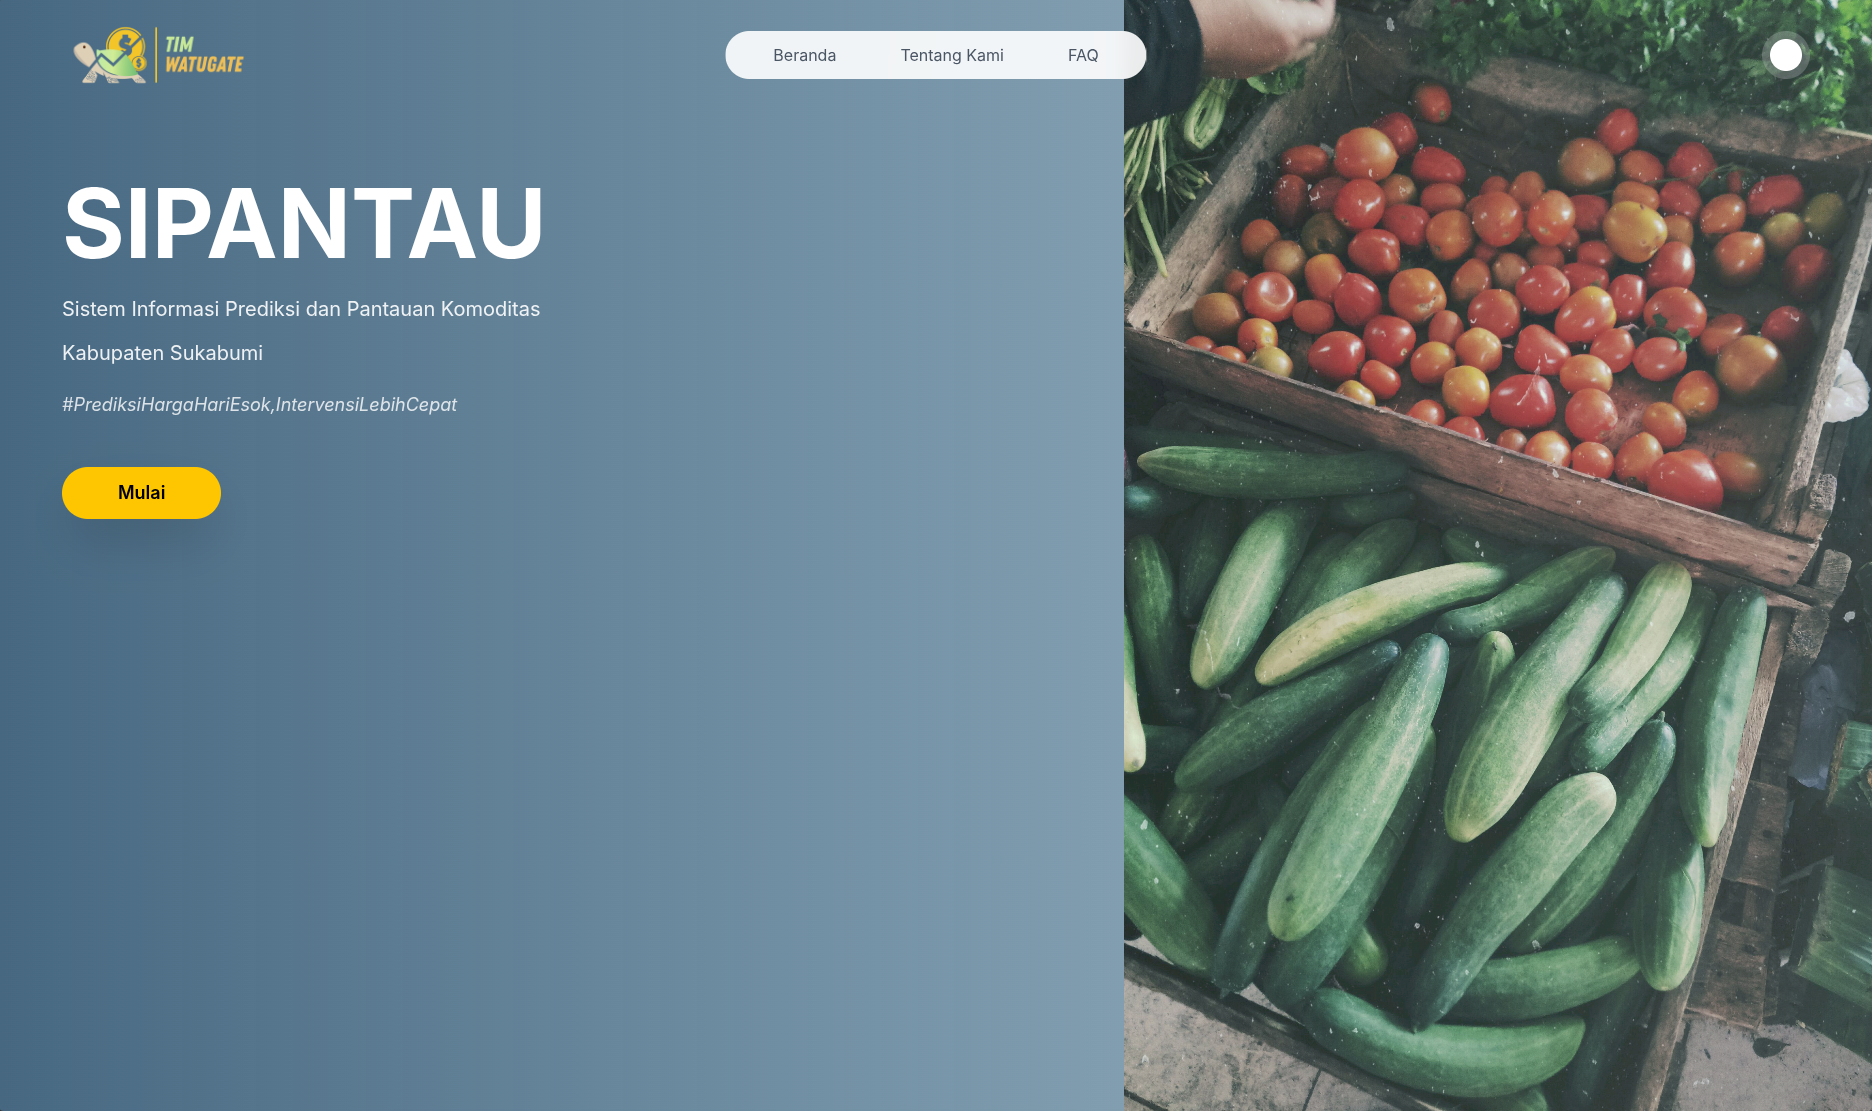
\includegraphics[width=0.75\textwidth]{img/fe-awal-lp.png}
    \caption{Kondisi awal frontend \textit{landing page} SIPANTAU}
    \label{fig:fe-awal-lp}
\end{figure}

\begin{figure}[ht]
    \centering
    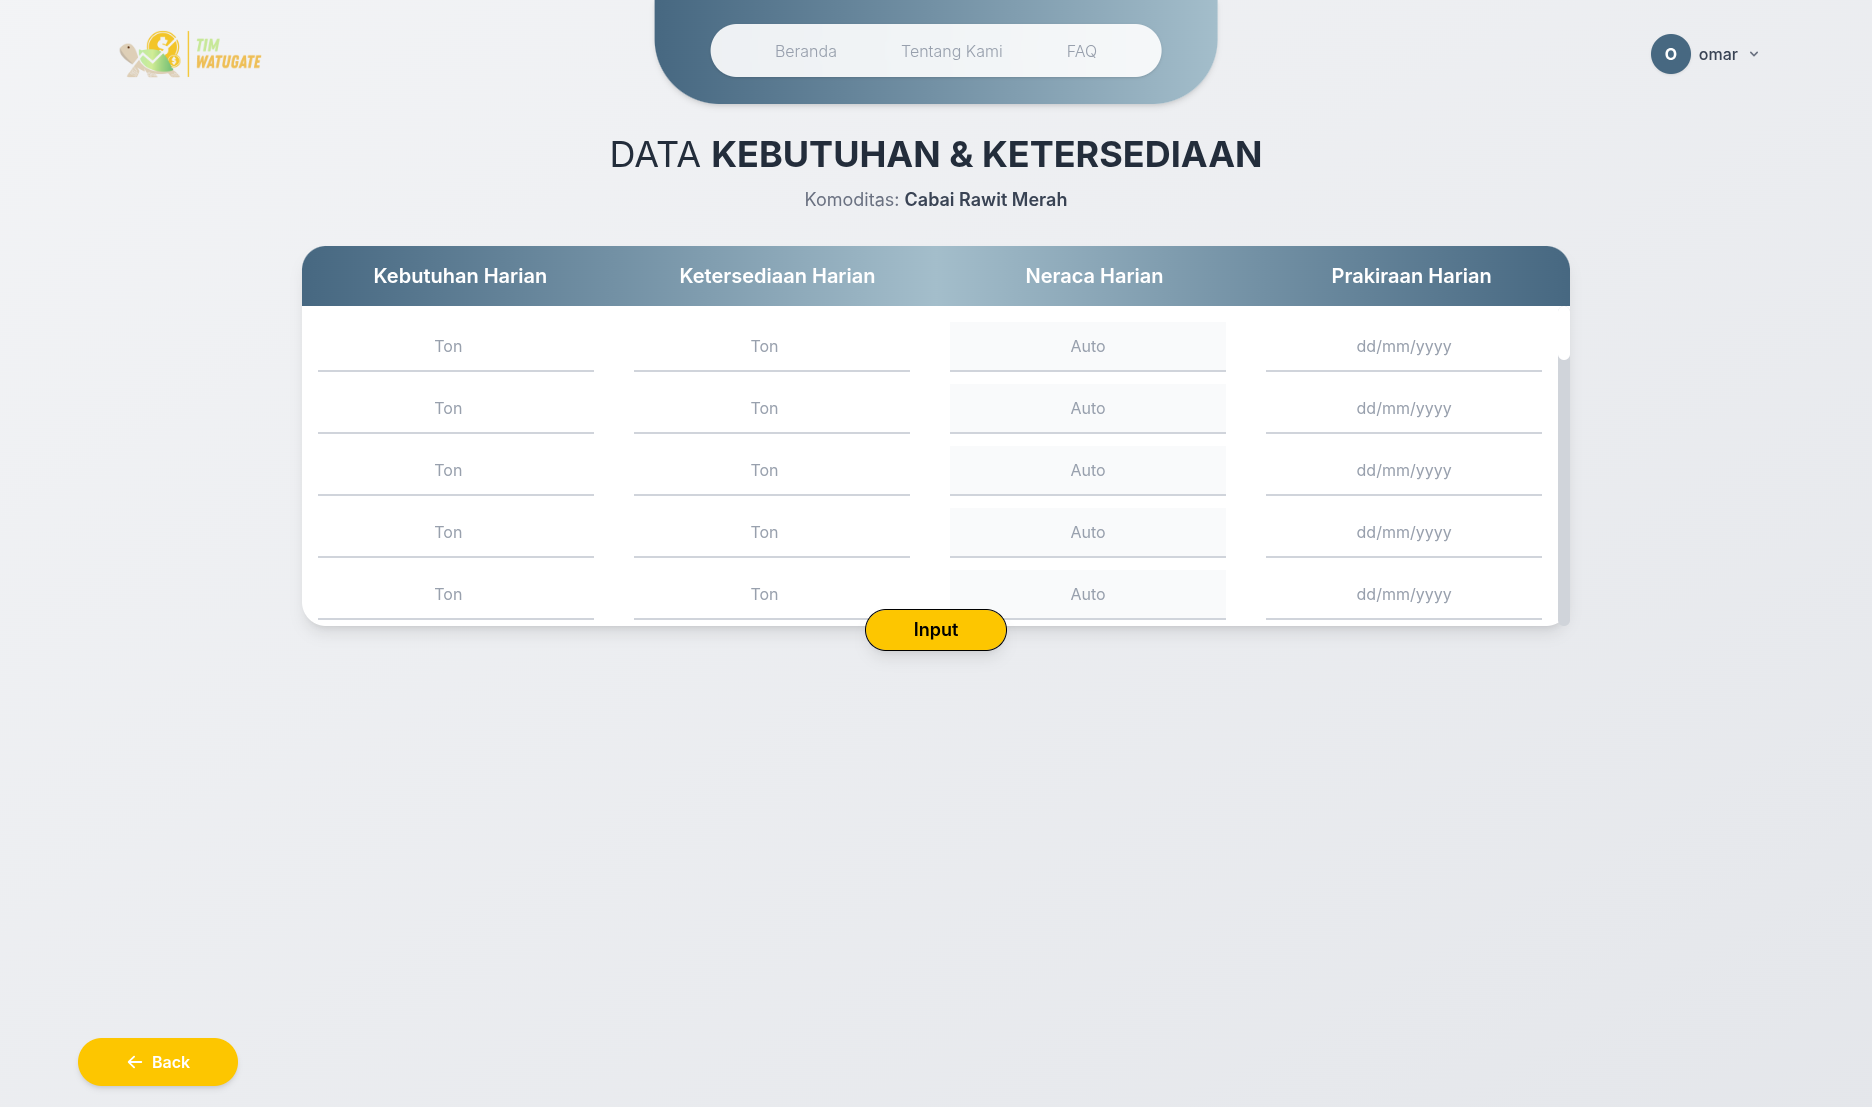
\includegraphics[width=0.75\textwidth]{img/fe-awal-input.png}
    \caption{Kondisi awal frontend halaman input data SIPANTAU}
    \label{fig:fe-awal-input}
\end{figure}

\begin{figure}[ht]
    \centering
    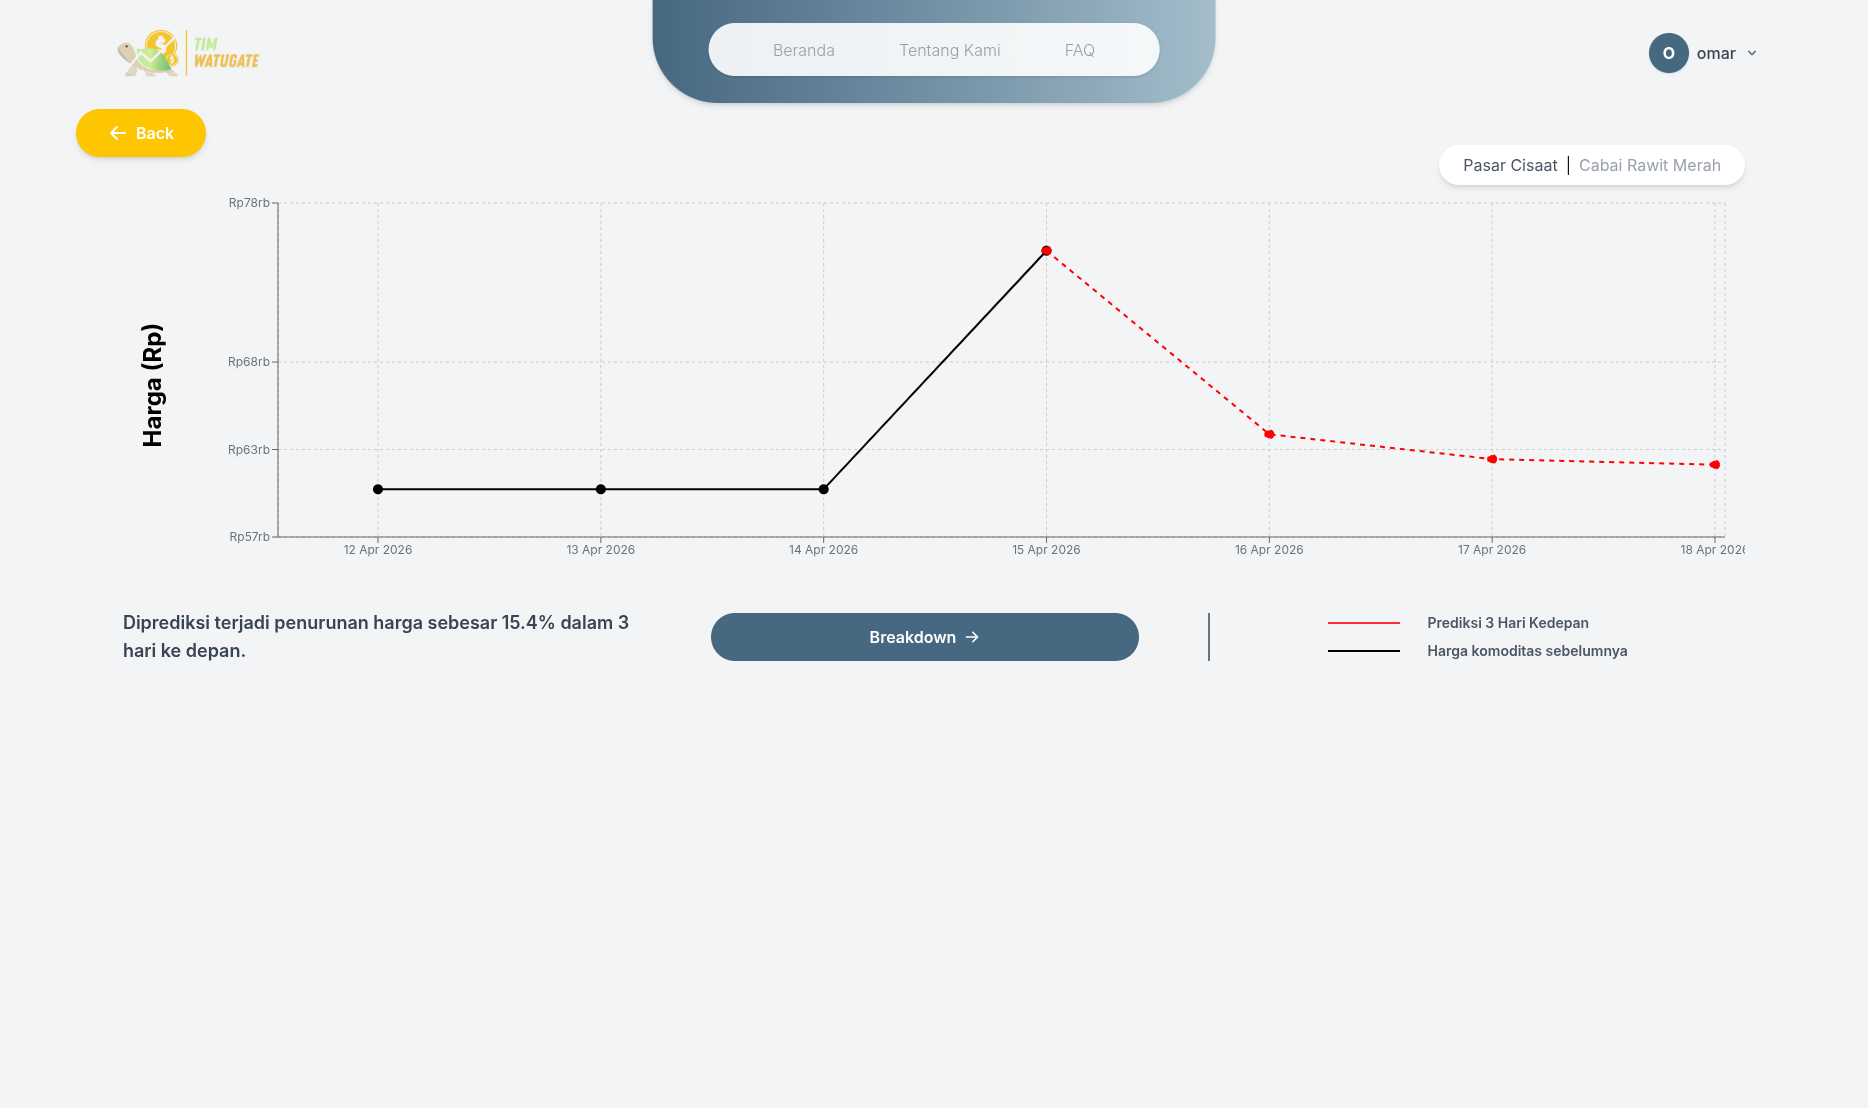
\includegraphics[width=0.75\textwidth]{img/fe-awal-prediksi.png}
    \caption{Kondisi awal frontend halaman prediksi SIPANTAU}
    \label{fig:fe-awal-prediksi}
\end{figure}

\begin{figure}[ht]
    \centering
    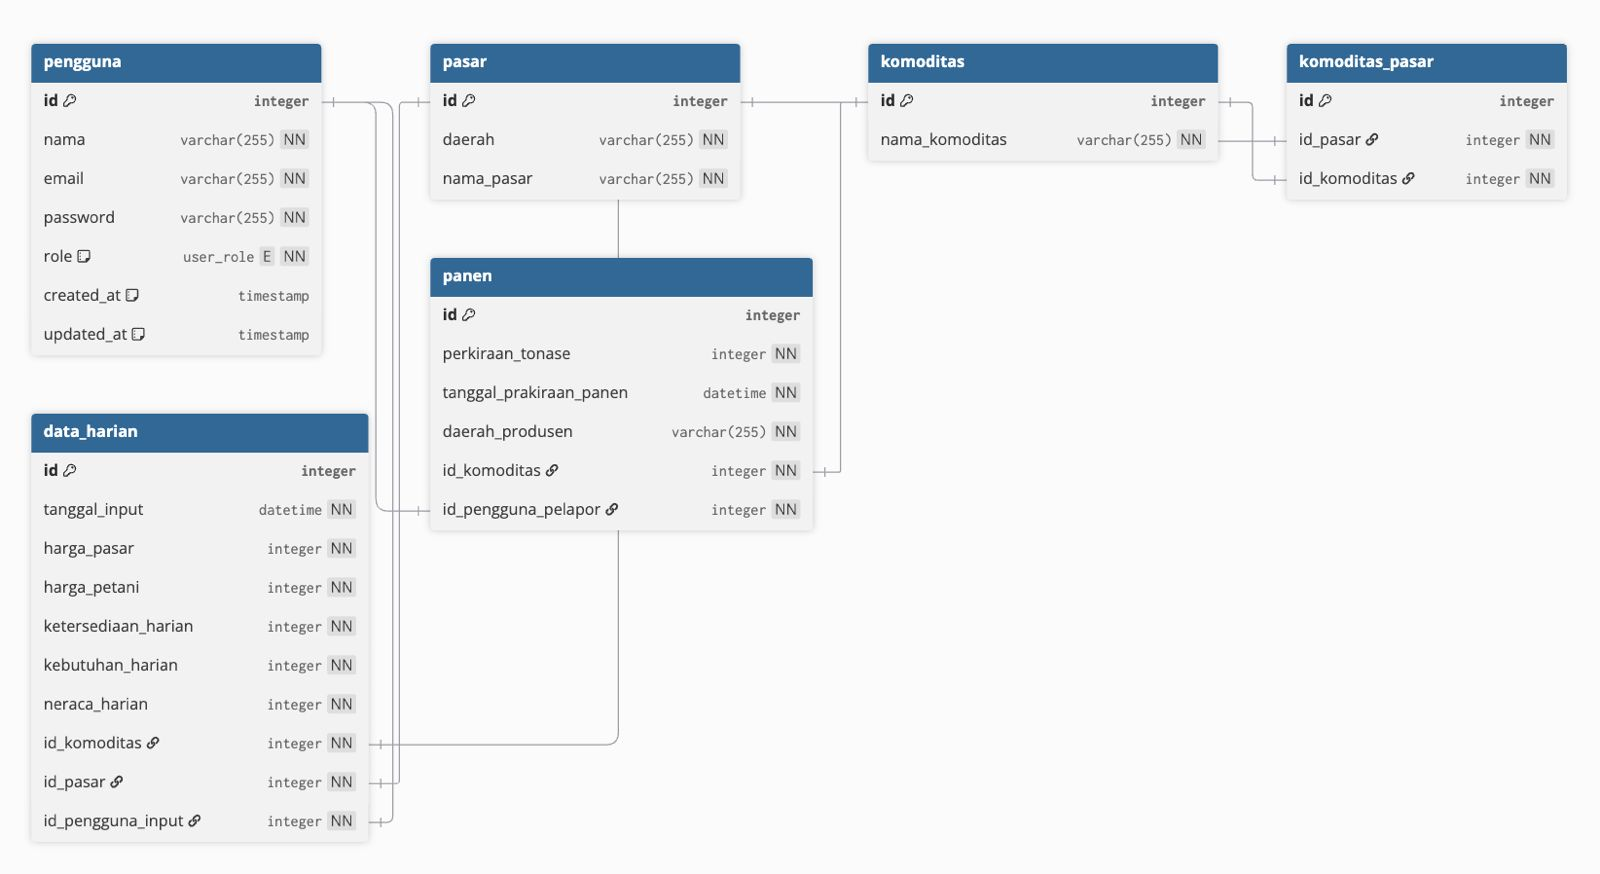
\includegraphics[width=0.75\textwidth]{img/db-awal.jpeg}
    \caption{Rancangan awal basis data SIPANTAU}
    \label{fig:db-awal}
\end{figure}

\FloatBarrier

Berdasarkan hasil identifikasi terhadap kondisi awal dan tujuan pengembangan SIPANTAU, diperoleh sejumlah kebutuhan fungsional yang harus dipenuhi oleh sistem. Kebutuhan tersebut mencakup mekanisme autentikasi dan otorisasi pengguna, pengelolaan data komoditas, penyediaan data melalui API, serta penyediaan fungsi prediksi harga komoditas. Kebutuhan fungsional yang diperoleh dari hasil analisis disajikan pada Tabel \ref{tab:kebutuhan-fungsional}.

\begin{longtable}{|c|c|p{5.0cm}|p{5.0cm}|}
    \caption{Kebutuhan fungsional SIPANTAU}
    \label{tab:kebutuhan-fungsional} \\
    \hline
    \textbf{No.} &
    \textbf{Kode} &
    \textbf{Kebutuhan Fungsional} &
    \textbf{Keterangan} \\
    \hline
    \endfirsthead

    \hline
    \textbf{No.} &
    \textbf{Kode} &
    \textbf{Kebutuhan Fungsional} &
    \textbf{Keterangan} \\
    \hline
    \endhead

    1 &
    KF-01 &
    Sistem dapat melakukan autentikasi pengguna. &
    Sistem melakukan verifikasi identitas pengguna sebelum pengguna mengakses fungsi yang memerlukan autentikasi. \\
    \hline

    2 &
    KF-02 &
    Sistem dapat melakukan otorisasi pengguna berdasarkan peran. &
    Sistem mengatur hak akses pengguna terhadap fungsi aplikasi berdasarkan peran yang dimiliki. \\
    \hline

    3 &
    KF-03 &
    Sistem dapat menerima dan mengelola data kebutuhan dan ketersediaan komoditas. &
    Pengguna yang memiliki hak akses dapat memasukkan dan mengelola data kebutuhan serta ketersediaan komoditas. \\
    \hline

    4 &
    KF-04 &
    Sistem dapat menerima dan mengelola data panen komoditas. &
    Pengguna yang memiliki hak akses dapat memasukkan dan mengelola data hasil panen komoditas. \\
    \hline

    5 &
    KF-05 &
    Sistem dapat menerima dan mengelola data harga petani. &
    Pengguna yang memiliki hak akses dapat memasukkan dan mengelola data harga komoditas pada tingkat petani. \\
    \hline

    6 &
    KF-06 &
    Sistem dapat menerima dan mengelola data harga pasar. &
    Pengguna yang memiliki hak akses dapat memasukkan dan mengelola data harga komoditas pada pasar. \\
    \hline

    7 &
    KF-07 &
    Sistem dapat menyediakan data melalui API. &
    Sistem menyediakan API yang memungkinkan data digunakan oleh komponen aplikasi yang membutuhkan. \\
    \hline

    8 &
    KF-08 &
    Sistem dapat menampilkan hasil prediksi harga komoditas untuk tiga hari ke depan. &
    Sistem menggunakan data historis yang diperlukan untuk memperoleh hasil prediksi harga melalui layanan model prediksi. \\
    \hline

\end{longtable}

Selain kebutuhan fungsional, hasil analisis juga mengidentifikasi beberapa kebutuhan non-fungsional yang berkaitan dengan batasan teknologi, keamanan, dan lingkungan operasional sistem. Pada awal pengembangan, teknologi yang digunakan pada \textit{frontend} telah ditetapkan menggunakan Next.js, sedangkan \textit{backend} ditetapkan untuk dikembangkan menggunakan Laravel. Selain itu, aspek keamanan dan penggunaan VPS yang telah disediakan juga menjadi batasan pengembangan sistem. Berdasarkan proses analisis dan perancangan, kebutuhan non-fungsional tersebut menjadi acuan dalam menentukan teknologi dan mekanisme implementasi aplikasi. Rincian kebutuhan non-fungsional SIPANTAU disajikan pada Tabel \ref{tab:kebutuhan-nonfungsional}.

\begin{longtable}{|c|c|p{5.0cm}|p{5.0cm}|}
    \caption{Kebutuhan non-fungsional SIPANTAU}
    \label{tab:kebutuhan-nonfungsional} \\
    \hline
    \textbf{No.} &
    \textbf{Kode} &
    \textbf{Kebutuhan Non-Fungsional} &
    \textbf{Keterangan} \\
    \hline
    \endfirsthead

    \hline
    \textbf{No.} &
    \textbf{Kode} &
    \textbf{Kebutuhan Non-Fungsional} &
    \textbf{Keterangan} \\
    \hline
    \endhead

    1 &
    KNF-01 &
    Sistem harus menerapkan keamanan pada aplikasi. &
    Sistem harus menerapkan mekanisme keamanan untuk melindungi akses dan komunikasi pada aplikasi. \\
    \hline

    2 &
    KNF-02 &
    Sistem harus dapat dideploy pada VPS yang telah disediakan. &
    Aplikasi harus dapat dijalankan pada lingkungan VPS yang disediakan sebagai lingkungan \textit{deployment}. \\
    \hline

    3 &
    KNF-03 &
    Pengembangan backend harus dapat diintegrasikan dengan frontend berbasis Next.js. &
    Backend yang dikembangkan harus menyediakan mekanisme komunikasi yang sesuai agar dapat digunakan oleh frontend yang telah dikembangkan menggunakan Next.js. \\
    \hline

    4 &
    KNF-04 &
    Backend harus dikembangkan menggunakan Laravel. &
    Pengembangan backend harus menggunakan framework Laravel sesuai dengan teknologi yang telah ditetapkan pada awal proyek. \\
    \hline

    5 &
    KNF-05 &
    Sistem harus menjaga konsistensi data. &
    Data yang disimpan dan diperbarui melalui aplikasi harus tetap konsisten dengan kondisi data pada basis data. \\
    \hline

\end{longtable}

Berdasarkan kebutuhan fungsional dan non-fungsional yang telah diidentifikasi, selanjutnya sistem dimodelkan untuk menggambarkan hubungan antara pengguna dengan fungsi yang tersedia pada SIPANTAU. Pemodelan tersebut menggambarkan aktor yang terlibat dalam sistem serta fungsi yang dapat dijalankan oleh masing-masing aktor sesuai dengan tanggung jawabnya. SIPANTAU memiliki lima aktor utama, yaitu Dinas Perdagangan, Dinas Ketahanan Pangan, Dinas Pertanian, Tim Pengendalian Inflasi Daerah (TPID), dan Admin.

Dinas Perdagangan menginput data harga pasar, sedangkan Dinas Ketahanan Pangan menginput data kebutuhan dan ketersediaan komoditas. Dinas Pertanian menginput data panen dan data harga komoditas pada tingkat petani. Ketiga perangkat daerah tersebut memperbarui data secara berkala agar sistem memiliki data yang mutakhir untuk mendukung proses prediksi harga komoditas.TPID menggunakan SIPANTAU untuk melihat hasil prediksi harga komoditas,sedangkan Admin memiliki akses terhadap seluruh fungsi sistem, termasuk melakukan registrasi akun pengguna.

Setiap aktor melakukan autentikasi sebelum mengakses fungsi yang memerlukan akses pengguna. Sistem menerapkan pembatasan hak akses berdasarkan peran pengguna sehingga setiap aktor hanya dapat menjalankan fungsi yang sesuai dengan kewenangannya. Hubungan antara aktor dan fungsi yang tersedia pada SIPANTAU ditunjukkan pada Gambar \ref{fig:use-case-sipantau}.

\begin{figure}[ht]
    \centering
    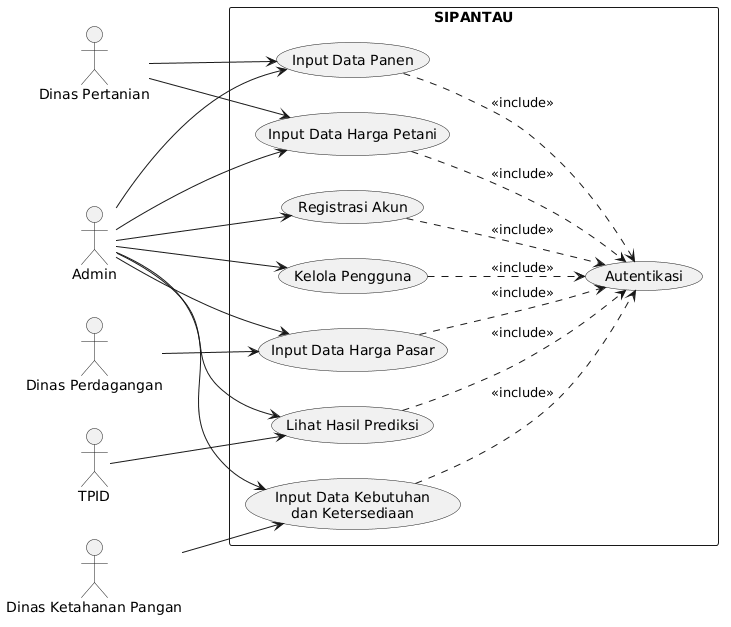
\includegraphics[width=0.75\textwidth]{img/use-case-sipantau.png}
    \caption{Use Case Diagram SIPANTAU}
    \label{fig:use-case-sipantau}
\end{figure}

Gambar \ref{fig:use-case-sipantau} menunjukkan pembagian fungsi SIPANTAU berdasarkan peran masing-masing aktor. Dinas Perdagangan mengelola data harga pasar, Dinas Ketahanan Pangan mengelola data kebutuhan dan ketersediaan, sedangkan Dinas Pertanian mengelola data panen dan harga petani. TPID melihat hasil prediksi harga komoditas, sedangkan Admin mengakses seluruh fungsi yang t   ersedia dan melakukan registrasi akun pengguna. Setiap aktor melakukan autentikasi sebelum mengakses fungsi sistem sesuai dengan hak akses yang dimilikinya.

Setelah hubungan antara aktor dan fungsi sistem ditentukan melalui Use Case Diagram, analisis dilanjutkan dengan menggambarkan alur aktivitas pada fungsi utama SIPANTAU. Activity Diagram menunjukkan urutan aktivitas yang dilakukan oleh pengguna dan komponen sistem dalam menjalankan setiap fungsi. Diagram tersebut mencakup proses autentikasi, registrasi akun, pengelolaan data, dan prediksi harga.

\begin{center}
    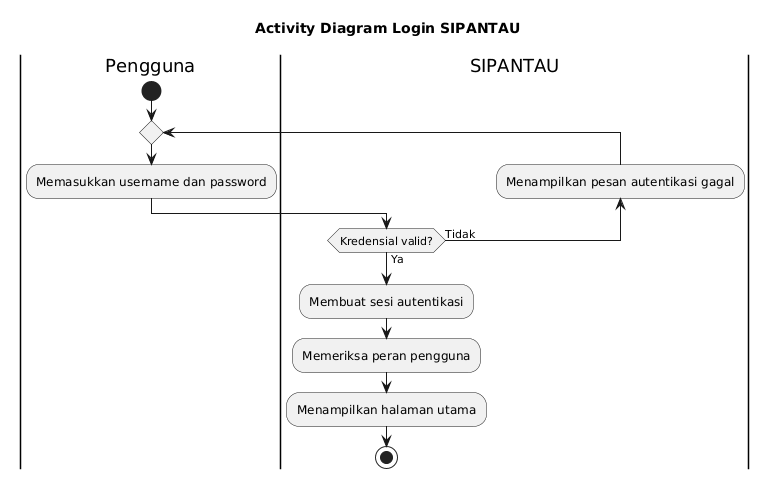
\includegraphics[width=0.8\textwidth]{img/ad-login.png}
    \captionof{figure}{Activity Diagram Autentikasi SIPANTAU}
    \label{fig:activity-login}
\end{center}

Activity Diagram autentikasi pada Gambar \ref{fig:activity-login} menggambarkan proses pengguna saat masuk ke SIPANTAU. Pengguna memasukkan username dan password, kemudian SIPANTAU memverifikasi kredensial tersebut. Sistem menampilkan pesan autentikasi gagal apabila kredensial tidak valid dan mengembalikan alur ke proses pengisian kredensial. Apabila kredensial valid, sistem membuat sesi autentikasi dan memeriksa peran pengguna sebelum menampilkan halaman utama. Alur tersebut memastikan bahwa pengguna telah terautentikasi sebelum mengakses fungsi yang tersedia pada sistem.

\begin{center}
    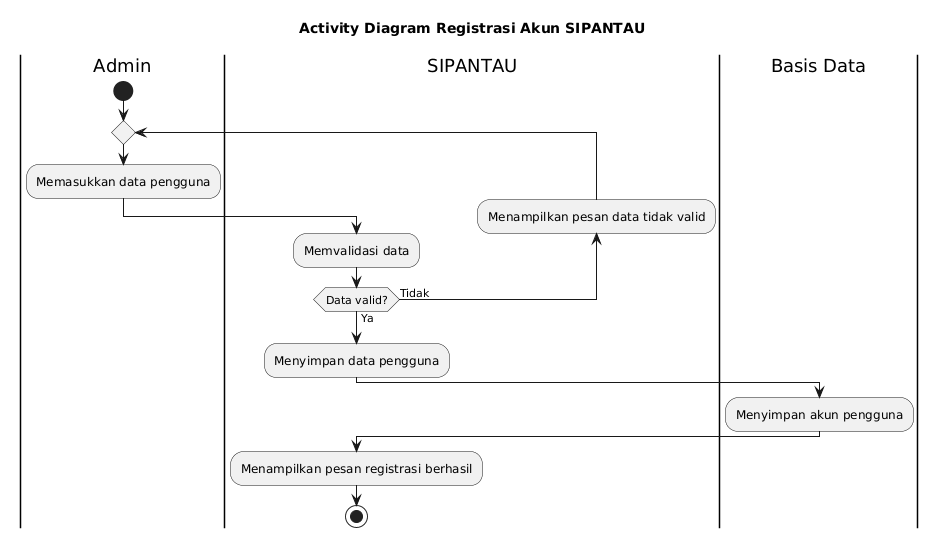
\includegraphics[width=0.8\textwidth]{img/ad-registrasi.png}
    \captionof{figure}{Activity Diagram Registrasi Akun SIPANTAU}
    \label{fig:activity-registrasi}
\end{center}

Activity Diagram registrasi akun pada Gambar \ref{fig:activity-registrasi} menggambarkan proses Admin dalam menambahkan akun pengguna ke SIPANTAU. Admin memasukkan data pengguna dan menentukan peran pengguna, kemudian SIPANTAU memvalidasi data tersebut sebelum menyimpannya. Sistem menampilkan pesan kesalahan apabila data tidak memenuhi validasi dan mengembalikan alur ke proses pengisian data. Apabila data valid, SIPANTAU menyimpan akun pengguna pada basis data dan menampilkan pesan bahwa proses registrasi berhasil.

\begin{center}
    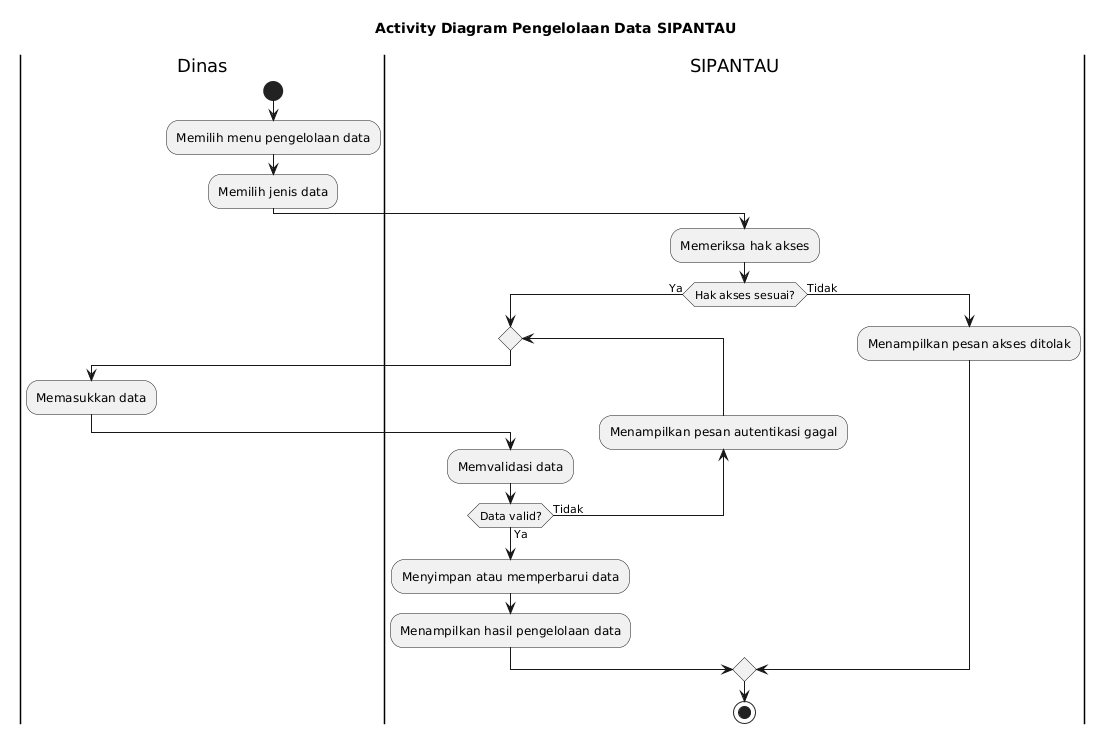
\includegraphics[width=0.8\textwidth]{img/ad-input.png}
    \captionof{figure}{Activity Diagram Pengelolaan Data SIPANTAU}
    \label{fig:activity-pengelolaan-data}
\end{center}

Activity Diagram pengelolaan data pada Gambar \ref{fig:activity-pengelolaan-data} menggambarkan proses Dinas dalam memasukkan dan mengelola data pada SIPANTAU. Dinas memilih menu dan jenis data yang sesuai dengan tanggung jawabnya, kemudian memasukkan data ke dalam sistem. SIPANTAU memeriksa hak akses pengguna sebelum memproses data dan melakukan validasi terhadap data yang dimasukkan. Sistem menampilkan pesan kesalahan apabila data tidak valid dan mengembalikan alur ke proses pengisian data. Apabila data telah memenuhi validasi, sistem menyimpan atau memperbarui data pada basis data dan menampilkan hasil pengelolaan data kepada pengguna.

\begin{center}
    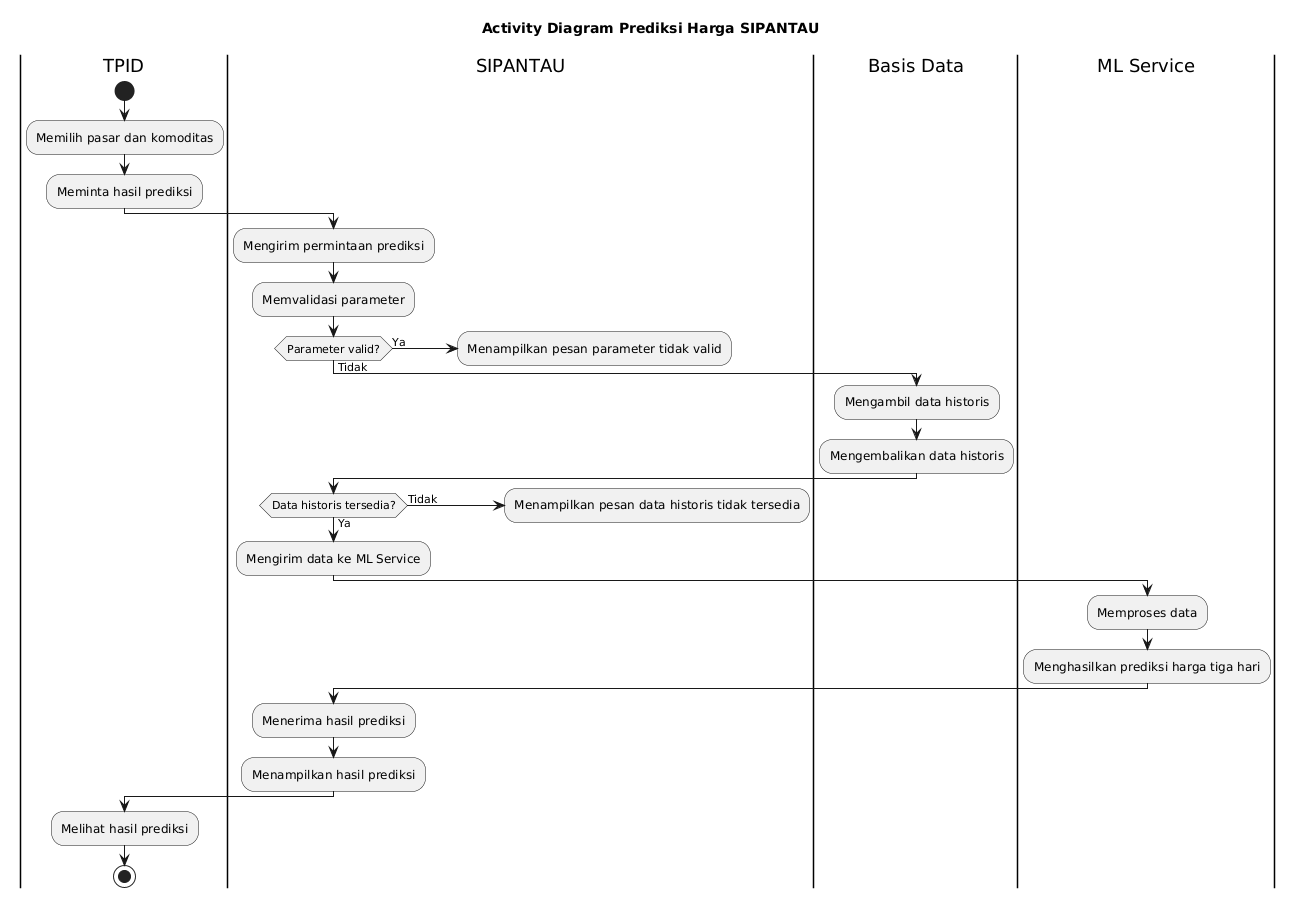
\includegraphics[width=0.8\textwidth]{img/ad-prediksi.png}
    \captionof{figure}{Activity Diagram Prediksi Harga SIPANTAU}
    \label{fig:activity-prediksi}
\end{center}

Activity Diagram prediksi harga pada Gambar \ref{fig:activity-prediksi} menggambarkan alur permintaan prediksi dari TPID hingga hasil prediksi ditampilkan. TPID memilih pasar dan komoditas, kemudian frontend mengirimkan permintaan prediksi kepada SIPANTAU. SIPANTAU memvalidasi parameter yang dikirimkan dan menampilkan pesan kesalahan pada frontend apabila parameter tidak valid. Setelah parameter valid, sistem mengambil data historis dari basis data dan memeriksa ketersediaan data tersebut.

Keempat Activity Diagram tersebut memperlihatkan alur utama yang perlu didukung oleh SIPANTAU berdasarkan kebutuhan yang telah diidentifikasi. Alur autentikasi memastikan pengguna dapat mengakses sistem sesuai dengan identitas dan perannya, sedangkan alur registrasi akun mendukung Admin dalam menyediakan akun bagi pengguna. Alur pengelolaan data mendukung pembaruan data komoditas oleh Dinas, sementara alur prediksi menghubungkan data historis dengan layanan model prediksi untuk menghasilkan prediksi harga. Hasil analisis tersebut menjadi dasar dalam menentukan rancangan basis data, arsitektur backend, mekanisme hak akses, integrasi layanan model prediksi, dan deployment aplikasi.

\subsection{Perancangan, Implementasi, dan Pengujian Backend dan Basis Data}

Bagian ini membahas hasil perancangan, implementasi, dan pengujian backend serta basis data SIPANTAU. Perancangan mencakup struktur basis data, arsitektur backend, dan penyediaan API untuk mendukung fungsi sistem yang telah ditetapkan. Implementasi kemudian merealisasikan rancangan tersebut menggunakan teknologi yang telah ditentukan, sedangkan pengujian dilakukan untuk memastikan fungsi backend dan basis data berjalan sesuai kebutuhan sistem.

\subsubsection{Perancangan}

Perancangan backend dan basis data dilakukan berdasarkan kebutuhan fungsional dan non-fungsional yang telah diidentifikasi pada tahap analisis. Perancangan tersebut mencakup struktur basis data, arsitektur backend, dan rancangan API yang digunakan untuk menyediakan dan mengelola data SIPANTAU.

Perancangan basis data menentukan struktur data dan hubungan antarentitas yang digunakan oleh SIPANTAU. Rancangan tersebut mencakup entitas pengguna, pasar, komoditas, harga pasar harian, harga petani harian, ketersediaan harian, dan panen. Hasil perancangan basis data SIPANTAU ditunjukkan pada Gambar \ref{fig:erd-sipantau}.

\begin{center}
    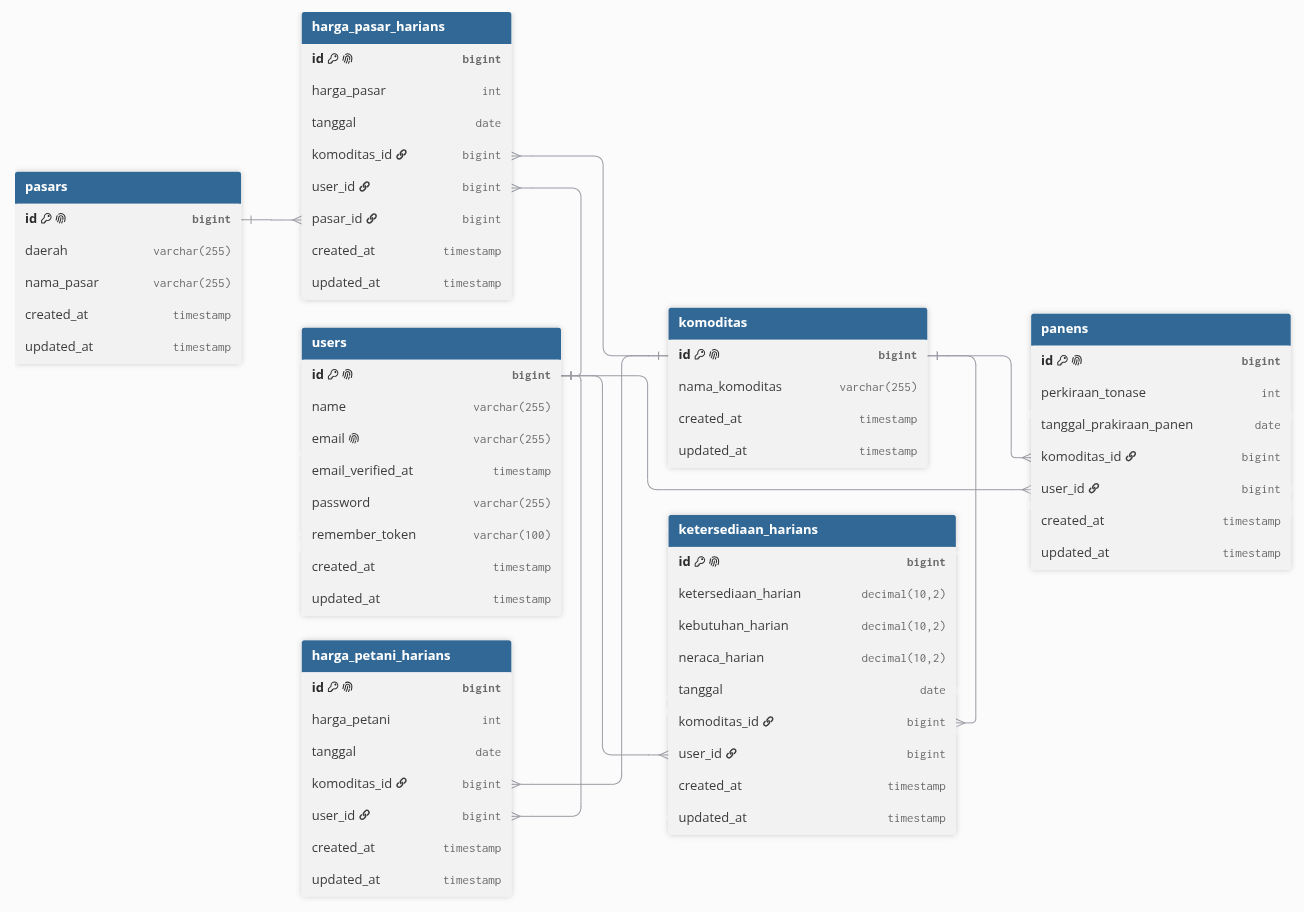
\includegraphics[width=\textwidth]{img/erd-sipantau.png}
    \captionof{figure}{Entity Relationship Diagram SIPANTAU}
    \label{fig:erd-sipantau}
\end{center}

Struktur basis data pada Gambar \ref{fig:erd-sipantau} menghubungkan data operasional dengan data referensi yang digunakan oleh SIPANTAU. Entitas \textit{komoditas} menjadi acuan bagi data harga pasar, harga petani, ketersediaan, dan panen, sedangkan entitas \textit{pasars} menjadi acuan bagi pencatatan harga pasar. Entitas \textit{users} terhubung dengan data yang dimasukkan oleh pengguna sehingga sistem dapat mencatat pengguna yang melakukan pengelolaan data.

\begin{longtable}{|c|p{4.1cm}|p{2.8cm}|p{2.3cm}|p{1.8cm}|}

    \caption{Relasi antartabel basis data SIPANTAU}
    \label{tab:relasi-database} \\

    \hline

    \multicolumn{1}{|c|}{\textbf{No.}} &
    \multicolumn{1}{c|}{\textbf{Tabel}} &
    \multicolumn{1}{c|}{\textbf{Kolom FK}} &
    \multicolumn{1}{c|}{
        \makecell[c]{\vspace{3pt}\textbf{Tabel}\\\textbf{Referensi}}
    } &
    \multicolumn{1}{c|}{
        \makecell[c]{\vspace{3pt}\textbf{Kolom}\\\textbf{Referensi}}
    } \\

    \hline
    \endfirsthead

    \hline

    \multicolumn{1}{|c|}{\textbf{No.}} &
    \multicolumn{1}{c|}{\textbf{Tabel}} &
    \multicolumn{1}{c|}{\textbf{Kolom FK}} &
    \multicolumn{1}{c|}{
        \makecell[c]{\vspace{3pt}\textbf{Tabel}\\\textbf{Referensi}}
    } &
    \multicolumn{1}{c|}{
        \makecell[c]{\vspace{3pt}\textbf{Kolom}\\\textbf{Referensi}}
    } \\

    \hline
    \endhead

    1 & \textit{harga\_pasar\_harians} & \textit{komoditas\_id} & \textit{komoditas} & \textit{id} \\ \hline
    2 & \textit{harga\_pasar\_harians} & \textit{user\_id} & \textit{users} & \textit{id} \\ \hline
    3 & \textit{harga\_pasar\_harians} & \textit{pasar\_id} & \textit{pasars} & \textit{id} \\ \hline
    4 & \textit{harga\_petani\_harians} & \textit{komoditas\_id} & \textit{komoditas} & \textit{id} \\ \hline
    5 & \textit{harga\_petani\_harians} & \textit{user\_id} & \textit{users} & \textit{id} \\ \hline
    6 & \textit{ketersediaan\_harians} & \textit{komoditas\_id} & \textit{komoditas} & \textit{id} \\ \hline
    7 & \textit{ketersediaan\_harians} & \textit{user\_id} & \textit{users} & \textit{id} \\ \hline
    8 & \textit{panens} & \textit{komoditas\_id} & \textit{komoditas} & \textit{id} \\ \hline
    9 & \textit{panens} & \textit{user\_id} & \textit{users} & \textit{id} \\ \hline

\end{longtable}

Tabel \ref{tab:relasi-database} menunjukkan hubungan antartabel yang digunakan dalam basis data SIPANTAU. Relasi tersebut menghubungkan data operasional dengan data pengguna dan data referensi yang diperlukan oleh sistem.

Perancangan backend selanjutnya menentukan struktur layanan yang mengelola proses bisnis SIPANTAU berdasarkan struktur basis data yang telah dirancang. Backend menggunakan Laravel untuk menerima dan memproses permintaan dari pengguna melalui frontend berbasis Next.js. Nginx digunakan sebagai API Gateway dan reverse proxy yang mengatur lalu lintas permintaan menuju layanan frontend dan backend. Backend Laravel berkomunikasi dengan basis data MySQL untuk mengelola data SIPANTAU dan berkomunikasi dengan ML Service berbasis FastAPI untuk menjalankan proses prediksi harga.

\begin{center}

    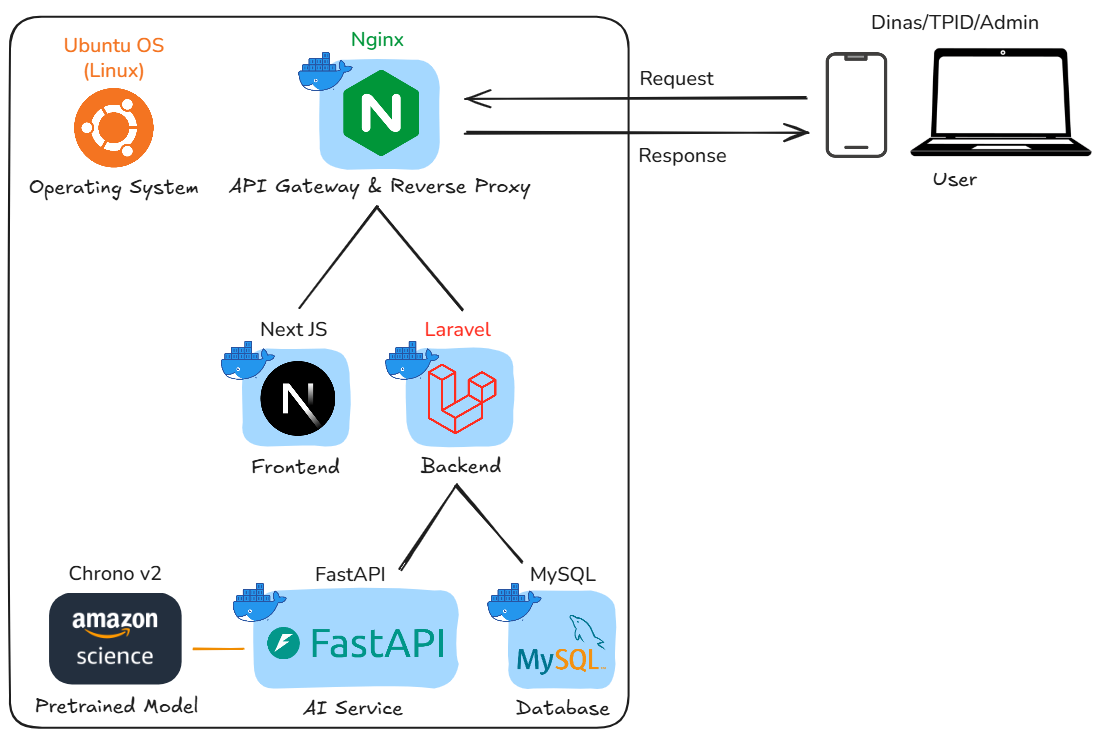
\includegraphics[width=1\textwidth]{img/arsitektur.png}

    \captionof{figure}{Arsitektur SIPANTAU}

    \label{fig:arsitektur-sipantau}

\end{center}

Arsitektur SIPANTAU pada Gambar \ref{fig:arsitektur-sipantau} menunjukkan hubungan antara komponen aplikasi yang digunakan dalam sistem. Sistem berjalan pada lingkungan Ubuntu yang menjadi sistem operasi tempat seluruh layanan aplikasi dijalankan. Nginx berperan sebagai API Gateway dan reverse proxy yang menerima permintaan dari pengguna dan meneruskannya kepada layanan yang sesuai. Frontend menggunakan Next.js untuk menyediakan antarmuka pengguna, sedangkan backend menggunakan Laravel untuk menangani proses bisnis dan menyediakan API.

Backend Laravel terhubung dengan basis data MySQL untuk menyimpan dan mengambil data yang digunakan oleh sistem. Backend juga terhubung dengan ML Service berbasis FastAPI untuk menjalankan proses prediksi harga. ML Service menggunakan model yang telah dilatih sebelumnya sebagai dasar proses prediksi. Dengan rancangan tersebut, proses pengelolaan data dan proses prediksi ditempatkan pada layanan yang terpisah sehingga masing-masing layanan dapat menjalankan tanggung jawabnya secara khusus.

Perancangan API selanjutnya menentukan endpoint yang digunakan untuk mendukung fungsi backend SIPANTAU dalam ruang lingkup pengembangan. Backend Laravel menyediakan endpoint untuk autentikasi pengguna, registrasi akun, pengelolaan data komoditas dan pasar, serta pengelolaan data ketersediaan, panen, harga pasar, dan harga petani.

\begin{longtable}{|c|c|p{3cm}|p{6.4cm}|}

    \caption{Rancangan endpoint API SIPANTAU}
    \label{tab:rancangan-api} \\

    \hline

    \textbf{No.} &
    \textbf{Method} &
    \textbf{Endpoint} &
    \textbf{Fungsi} \\

    \hline
    \endfirsthead

    \hline

    \textbf{No.} &
    \textbf{Method} &
    \textbf{Endpoint} &
    \textbf{Fungsi} \\

    \hline
    \endhead

    1 & POST & \texttt{/login} &
    Melakukan autentikasi pengguna. \\ \hline

    2 & POST & \texttt{/logout} &
    Mengakhiri sesi autentikasi pengguna. \\ \hline

    3 & GET & \texttt{/me} &
    Mengambil informasi pengguna yang sedang terautentikasi. \\ \hline

    4 & POST & \texttt{/register} &
    Mendaftarkan akun pengguna baru. \\ \hline

    5 & GET & \texttt{/komoditas} &
    Mengambil data komoditas. \\ \hline

    6 & POST & \texttt{/komoditas} &
    Menambahkan data komoditas baru. \\ \hline

    7 & GET & \texttt{/pasar} &
    Mengambil data pasar. \\ \hline

    8 & POST & \texttt{/pasar} &
    Menambahkan data pasar baru. \\ \hline

    9 & POST & \texttt{/ketersediaan} &
    Menyimpan data ketersediaan dan kebutuhan harian komoditas. \\ \hline

    10 & GET & \texttt{/ketersediaan} &
    Mengambil data ketersediaan harian. \\ \hline

    11 & POST & \texttt{/panen} &
    Menyimpan data perkiraan panen komoditas. \\ \hline

    12 & GET & \texttt{/panen} &
    Mengambil data panen. \\ \hline

    13 & POST & \texttt{/harga-pasar} &
    Menyimpan data harga pasar harian. \\ \hline

    14 & GET & \texttt{/harga-pasar} &
    Mengambil data harga pasar harian. \\ \hline

    15 & POST & \texttt{/harga-petani} &
    Menyimpan data harga petani harian. \\ \hline

    16 & GET & \texttt{/harga-petani} &
    Mengambil data harga petani harian. \\ \hline

\end{longtable}

Tabel \ref{tab:rancangan-api} menunjukkan endpoint API yang digunakan untuk mendukung pengelolaan data pada SIPANTAU. Endpoint tersebut menyediakan operasi untuk menyimpan dan mengambil data yang digunakan oleh sistem.

\section{Pembahasan}

% -----------------------------------------------------------------
% Bibliography
% -----------------------------------------------------------------
% -- \addcontentsline{toc}{chapter}{DAFTAR PUSTAKA}
\begingroup
\emergencystretch=3em
\sloppy
\printbibliography[title={DAFTAR PUSTAKA}]
\endgroup


\end{document}
